\chapter{Экспериментальное исследование оптических частотных гребенок в кристаллических микрорезонаторах} \label{chapt3}

\section{Изготовление кристаллических микрорезонаторов методом алмазного точения}

В литературе были продемонстрированы следующие способы изготовления микрорезонаторов:

\begin{itemize}
  \item Плавление в пламени водородной горелки для микросфер из плавленого кварца.
  \item Выжигание мощным лазером $CO_2$ вращающейся заготовки.
  \item Механическое точение резонаторов
  \item Различные литографические методы для изготовление интегральных микрорезонаторов
\end{itemize}

В данной работе для изговтовления всех микрорезонаторов из кристаллических материалов изучаося и использовался метод алмазного точения с последующей полировкой алмазными суспензиями.

Общий внешний микрорезонаторов представлен на рис. \ref{cavity_scheme_big}. Основные характеристики микрорезонатора - это диаметр, толщина цилиндра и радиус закругления боковой поверхности цилиндра, где сосредоточено поле мод шепчущей галереи.  Размеры варьируются в следующих пределах: диаметр от 100 мкм – 8 мм (в зависимости от необходимой ОСД $FSR= \frac{c}{2\pi Rn}$), толщина 0.1 мм – 2мм (в зависимости от толщины изначальной заготовки) и радиус закругления от 30 мкм до $R/2$ (где $R$ – радиус резонатора).

\begin{figure}[ht]
    \centering
  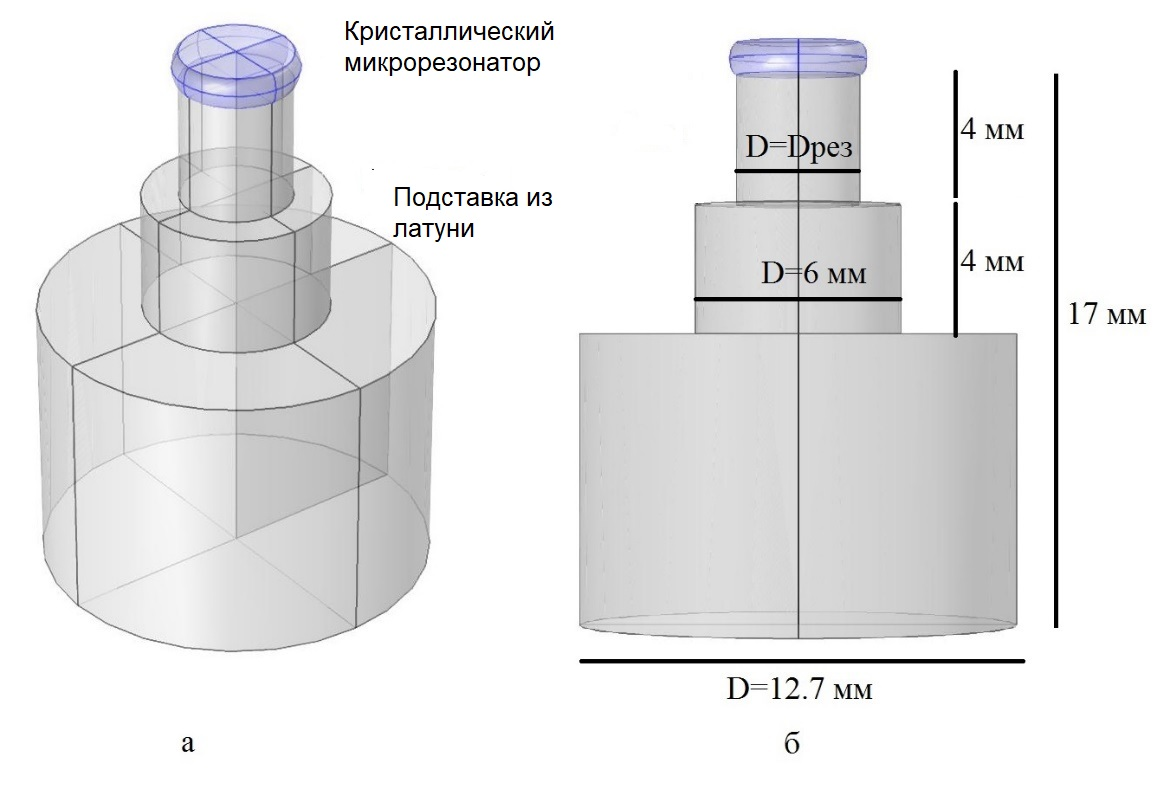
\includegraphics[width=0.5\linewidth]{cavity_scheme_big}
  \caption{Внешний вид кристаллического микрорезонатора и пьедестала: а – 3D вид, б – сечение XZ}
  \label{cavity_scheme_big}
\end{figure}

Для изготовления микрорезонатора с модами шепчущей галереи (ММШГ) использовались кристаллические пластины фторида магния ($MgF_2$), фторида кальция ($CaF_2$), фторида бария ($BaF_2$), фторида стронция ($SrF_2$), фторида лития ($LiF$), ниобата лития ($LiNbO_3$), танталата лития ($LiTaO_3$), кремния ($Si$), кристаллического кварца ($SiO_2$) и ряда других матералов.

Кристаллические микрорезонаторы из вышеуказанных материалов не могут быть изготовлены путем нагрева и обжига пламенем или мощным $СО_2$ лазером. Также пока не разработаны литографические способы их изготовления с необходимым качеством поверхности. Поэтому используется механическая обработка заготовок кристаллов в два этапа: точение алмазным резцом на прецизионном станке и последующая полировка алмазными пленками и суспензиями.

Ниже приведена последовательность действий, необходимых для изготовления микрорезонатора:

\begin{itemize}
  \item Наклеивание цилиндрической заготовки кристалла на латунную подставку с помощью УФ клея.
  \item Вытачивание цилиндра заданного диаметра алмазным резцом на станке алмазного точения (может выполняться изношенным резцом).
  \item Вытачивание на цилиндре микрорезонатора с заданной геометрией с помощью острого алмазного резца и программы для ЧПУ
  \item Очистка микрорезонатора с помощью салфетки, смоченной в изопропаноле или метаноле
  \item Проверка качества получившейся поверхности в микроскоп для обнаружения возможных шероховатостей, а также с помощью профилометра и методом проверки добротности
\end{itemize}

Хотя техника алмазного точения единственной точкой (SPDT, single point diamond turning) давно используется в большом количестве приложений, строгой теории для оптимального процесса точения нет. В процессе работы были экспериментально найдены оптимальные параметры для процесса точения.

Для алмазного точения использовался прецизионный станок с ЧПУ DAC ALM Lathe (рис. \ref{lathe}). Станок имеет прецизионный шпиндель на воздушных подшипниках и $2$ подвижные оси X,Y также на воздушных подшипниках. Точность подачи Х,Y специфицирована в $<10$ нм. Станок управляется с помощью программ, написанных на специально разработанном языке DSL. Станок оборудован высокоточным датчиком расстояния (LVDT), который измеряет расстояние по оси Y до момента касания заготовки. Также в комплекте к станку идет датчик высоты (профилометр), который измеряет изменение высоты с точностью до $0.1$ мкм. При двустороннем точении используется датчик, наносящий тонкие угловые отметки, позволяющие калибровать начало отсчета по оси C (угловое вращение шпинделя). Станок оборудован осциллирующим резцом, который синхронизируется с вращением шпинделя, и позволяет изготавливать асферические поверхности, а также выступы на фронтальной поверхности заготовки.

\begin{figure}[ht]
  \begin{minipage}[ht]{0.49\linewidth}\centering
    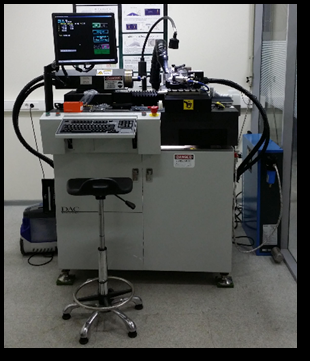
\includegraphics[width=1\linewidth]{lathe}
  \end{minipage}
  \hfill
  \begin{minipage}[ht]{0.49\linewidth}\centering
    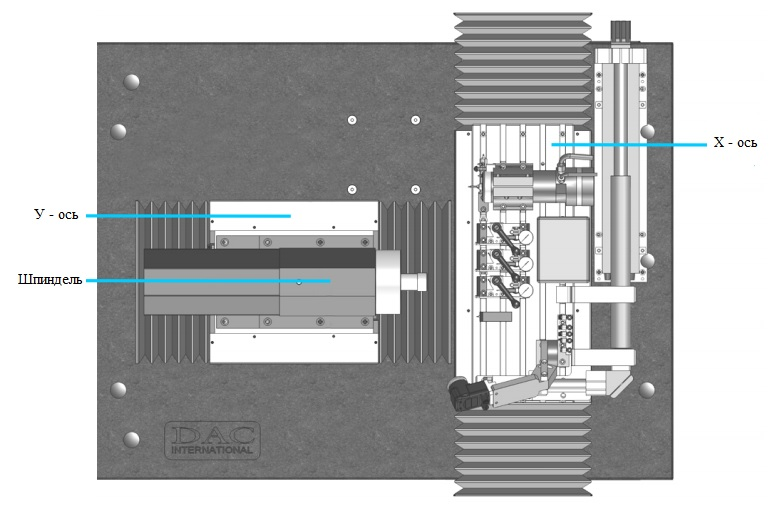
\includegraphics[width=1\linewidth]{lathe_top_view}
  \end{minipage}
  \caption{Прецизионный станок алмазного точения DAC ALM Lathe. Направление осей X,Y.}
  \label{lathe}
\end{figure}

Для точения использовались поликристаллические алмазные резцы производства KY Diamonds следующих типов (рис. \ref{diamond_tools}): 1) с радиусом кривизны 500 мкм, рабочей дугой окружности в 120 градусов, с 0 углом наклона рабочего края, конический задний угол резца 10 градусов; 2) с радиусом кривизны 100 мкм, рабочей дугой окружности в 60 градусов, с -25 углом наклона рабочего края, цилиндрический задний угол резца 8 градусов; 3) острый резец невыдержанным радиусом кривизны 4 мкм, 0 угол наклона рабочего края. Резцы располагались в держателе перпендикулярно (или под углом 80 градусов) оси вращения шпинделя со вставленным резонатором.

\begin{figure}[ht]
  \begin{minipage}[ht]{0.24\linewidth}\centering
    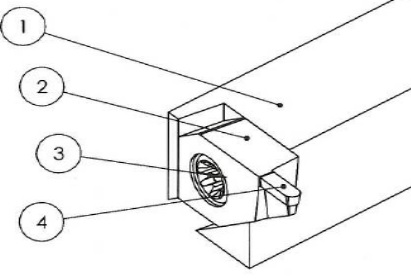
\includegraphics[width=1\linewidth]{tool1}
  \end{minipage}
  \hfill
  \begin{minipage}[ht]{0.24\linewidth}\centering
    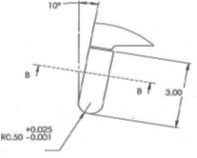
\includegraphics[width=1\linewidth]{tool2}
  \end{minipage}
  \hfill
  \begin{minipage}[ht]{0.24\linewidth}\centering
    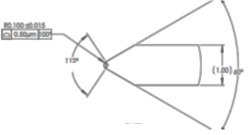
\includegraphics[width=1\linewidth]{tool3}
  \end{minipage}
  \hfill
  \begin{minipage}[ht]{0.24\linewidth}\centering
    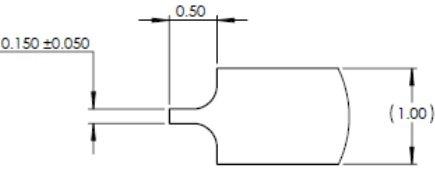
\includegraphics[width=1\linewidth]{tool4}
  \end{minipage}
  \caption{Чертежи используемых резцов.}
  \label{diamond_tools}
\end{figure}

Калибровка резцов проводилась по следующей методике:

\begin{itemize}
    \item В цангу вставляется заготовка (пластиковый цилиндр) диаметром 12.7 мм. Шпиндель подводится к калибруемому резцу. Выставляется на глаз отступ по оси Y до момента появления стружки (касания алмазного резца).
    \item Запускается программа, которая датчиком измеряет расстояние между фронтальной рабочей поверхностью до и после снятия слоя заданной толщины (например, 50 мкм). Точно зная это расстояние, окончательно калибруется зазор между датчиком расстояния LVDT и рабочей точкой резца.
    \item Запускается программа, наносящая штрих глубиной 1 мкм от края заготовки до ее центра (без вращения шпинделя). В оптический микроскоп (увеличение 40x) измеряется расстояние от центра заготовки до штриха (рис. \ref{tool_calibration}). Для правильной калибровки рабочая кромка резца изначально должна быть немного ниже центра. Используя датчик высоты, подстраивается высота калибруемого резца. Процедура повторяется до тех пор, пока штрих не будет проходить строго через центр заготовки.
    \item Проводится автоматическая калибровка расстояния по оси Х от рабочей точки алмазного резца до центра заготовки путем вытачивания трех концентрических окружностей: две при вращении шпинделя по часовой стрелке с одной стороны от центра, третья при вращении шпинделя в обратную сторону с другой стороны от центра. Далее измеряется получившееся расстояние между этими окружностями (с помощью датчика LVDT) и корректируется величина отступа между рабочей точкой резца и центром заготовки по оси X.
    \item В конце проводится калибровка расстояния по оси X до рабочей точки резца при точении цилиндра. Важно отметить, что точение фронтальной поверхности заготовки (перпендикулярно оси вращения шпинделя) и точение боковой поверхности цилиндра (параллельно оси вращения) осуществляется разными точками. Калибровка проводится путем вытачивания цилиндра заданного диаметра с последующим измерением получившегося диаметра с помощью микрометра. При необходимости расстояние по оси Х корректируется, и калибровка повторяется. Стоит подчеркнуть, что эта калибровка наименее точная из всех, т.к. погрешность микрометра при измерении диаметра цилиндра из мягкого пластика может составлять 3-5 мкм.
\end{itemize}


\begin{figure}[ht]
    \centering
  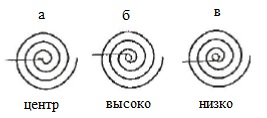
\includegraphics[width=0.5\linewidth]{tool_calibration}
  \caption{Результат калибровки высоты резца (правильная калибровка, резец высоко, резец низко).}
  \label{tool_calibration}
\end{figure}

Калибровка резцов осуществляется после каждой смены алмаза или при значительных дефектах обрабатываемых поверхностей.
Перед точением на станке из большой пластины материала резонатора вырезаются заготовки прямоугольной формы нужного малого размера. Для этого используется пила с алмазным диском, охлаждение производится водой.
Далее кристаллические заготовки наклеиваются на держатель (пьедестал) из пластика диаметром 12,7 мм, который соответствуют диаметру цанги на шпинделе станка. В работе использовались оптические клеи от производителя Norland Products (марки NOA 60, 61, 63, 65, 68), которые отвердевают при облучении УФ лампой. Клеи отличаются вязкостью в жидком виде, модулем упругости и твердостью в затвердевшем виде, оптическим показателем преломления и областью прозрачности. Все они не являются токопроводящими. Наилучший результат был достигнут с марками NOA 61, 65. Время облучения УФ лампой на длине 365 нм и мощностью 27 Вт/см$^2$ составляло 10 мин. Также использовались эпоксидная смола и этилцианакрилат, которые также давали хороший результат, но не позволяли долго центровать кристаллическую заготовку. Минимальный диаметр микрорезонатора, при котором не происходило отклеивание при точении, составил 700 мкм.
УФ клеи удобны для фиксации элементов ММШГ в крепежной сборке, т.к. позволяют юстироваться необходимое время и при отвердевании под УФ лампой не меняют свои размеры. После точения микрорезонаторы переклеивались на пьедестал меньшего диаметра или в крепежную сборку негабаритного макета. Все клеи размягчались и позволяли отклеить микрорезонатор при нагреве до 300-400 С. Также были испытаны двухкомпонентные клеи AremCo, который отвердевают за 24 часа при температуре 94 С, и выдерживают температуру нагревания до 400 С. Такой клей может использоваться при отжиге резонаторов.

Для центровки кристаллической заготовки в пластиковом пьедестале вырезалось отверстие глубиной 0.5 мм и диаметром, позволяющим разместить в нем заготовку. В отверстие заливался клей, помещалась заготовка и облучалась УФ лампой. Проверка центровки и перпендикулярности плоскости кристалла и оси вращения шпинделя проводилась визуально с помощью микроскопической трубы, подвешенной над шпинделем станка.

Были написаны программы на языке DAC DSL для вытачивания из цилиндрических кристаллических заготовок микрорезонаторов ММШГ со следующими профилями боковой поверхности: угловая, сферическая, прямоугольный выступ (рис. \ref{cavity_fab,cavity_small}). Параметры геометрии микрорезонатора настраиваются в широком диапазоне, ограниченном в основном геометрией самого алмазного резца.


\begin{figure}[ht]
  \begin{minipage}[ht]{0.49\linewidth}\centering
    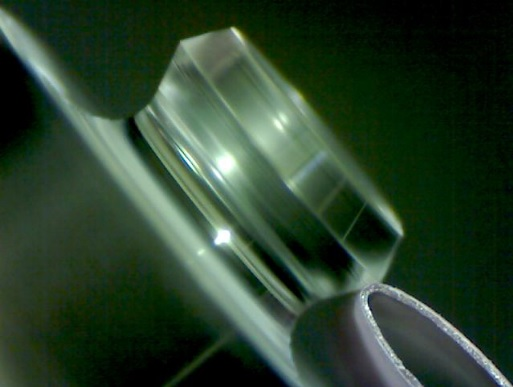
\includegraphics[width=1\linewidth]{cavity_fab_pad}
  \end{minipage}
  \hfill
  \begin{minipage}[ht]{0.49\linewidth}\centering
    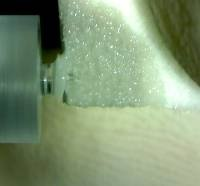
\includegraphics[width=1\linewidth]{cavity_fab_polishing}
  \end{minipage}
  \caption{Процесс ручной полировки алмазной шкуркой (слева) и алмазной суспензией (справа). Чистка резонатора проводилась на том же устройстве с использованием метилового спирта и салфеток Kimwipes.}
  \label{cavity_fab}
\end{figure}

\begin{figure}[ht]
\centering
  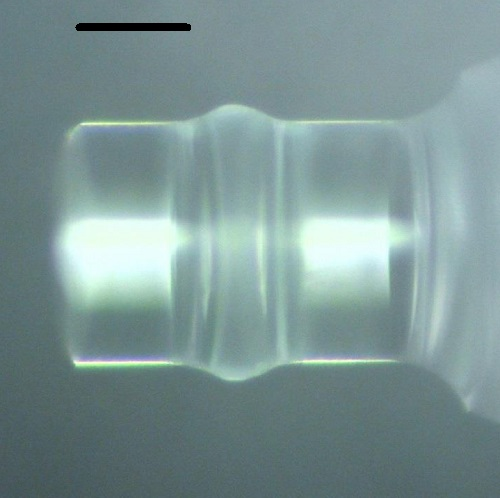
\includegraphics[width=0.5\linewidth]{cavity_fab_small}
  \caption{Микрорезонатор ММШГ ($MgF_2$) диаметром 250 мкм и радиусом кривизны боковой поверхности 50 мкм, выточенный с помощью программы DAC DSL.}
  \label{cavity_small}
\end{figure}

Алгоритм работы программы следующий:
\begin{itemize}
  \item Задаются начальные параметры (см рис. \ref{cavity_scheme})
  \begin{enumerate}
    \item диаметр заготовки (\texttt{blank\_diameter}),
    \item конечный внешний диаметр микрорезонатора (\texttt{diameter}),
    \item отступ от фронтальной (левой по рис. 32) поверхности (\texttt{front\_margin}), чтобы избежать возможных сколов у края
    \item хорда (\texttt{chord}), на которой располагается боковой выступ с радиусом кривизны (\texttt{curvature\_radius})
    \item высота (толщина) микрорезонатора ММШГ (\texttt{blank\_thickness})
    \item обороты шпинделя (\texttt{rpm})
    \item скорость движения резца при точении цилиндра (\texttt{cylinder\_fr}) и финального прохода с кривизной боковой поверхности (\texttt{fr})
    \item глубина захода резки при точении цилиндра (\texttt{cylinder\_step}) и финального прохода с кривизной боковой поверхности (\texttt{step\_amount\_to\_remove}).
  \end{enumerate}
  \item Грубым резцом стачивается цилиндр до нужного диаметра (направление движение резца параллельно оси вращения шпинделя) путем стачивания слоев высотой \texttt{cylinder\_step} со скоростью \texttt{cylinder\_fr}
  \item Финальным чистовым резцом (с радиусом кривизны алмаза, выдержанным с точностью 25 нм) последовательно стачиваются слои высотой \texttt{step\_amount\_to\_remove} с выступом сферической формы, передним отступом (\texttt{front\_margin}) и кривизной (\texttt{curvature\_radius}). Используется скорость движения резца \texttt{fr}.
\end{itemize}

\begin{figure}[ht]
\centering
  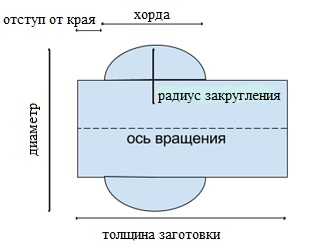
\includegraphics[width=0.5\linewidth]{cavity_scheme}
  \caption{Рисунок микрорезонатора ММШГ с параметрами для программы DAC DSL алмазного точения.}
  \label{cavity_scheme}
\end{figure}

Основными параметрами, влияющими на качество изготавливаемых микрорезонаторов ММШГ, являются скорость вращения шпинделя (rpm), линейная скорость точения (угловая скорость шпинделя умноженная на радиус резонатора), скорость движения резца (feed rate) и глубина захода (depth of cut). Опытным путем были определены следующие оптимальные параметры для точения кристаллов $MgF_2, CaF_2, BaF_2, LiNbO_3, LiTaO_3$:

\begin{itemize}
    \item rpm=400-1500;
    \item \texttt{feed\_rate}=2-3 мкм/оборот для предварительной обработки и <1-2 мкм/оборот для финального прохода;
    \item \texttt{depth\_of\_cut}=2-5 мкм для грубой обработки и 0.05-0.5 мкм для финального прохода.
\end{itemize}

Важнейшим фактором является охлаждение во время точения. Для этого на резец и резонатор распыляется охлаждающая жидкость, которая сразу же отсасывается в воздухозаборник вместе со срезанными стружками. В качестве охлаждения использовался изопропиловый спирт или Exxsol D100 – деароматизированная углеводородная жидкость. Жидкость не должна попадать внутрь шпинделя или линейных подач X,Y, а также должна быстро улетучиваться и не оставлять следов на кристалле. Без использования жидкости точение возможно, но с минимальной глубиной и скоростью подачи, при этом алмаз изнашивается значительно быстрее, а качество поверхности выточенного резонатора получается хуже.

После точения проводилась очистка микрорезонатора от кристаллической стружки с помощью полимерных салфеток, смоченных в метаноле. Сразу из-под резца получается добротность $10^5 -- 10^6$. Дальнейшее увеличение добротности достигается последовательной ручной полировкой с помощью и алмазных суспензий с уменьшающимся размером зерна (2.5 - 1 - 0.5 - 0.25 - 0.1 – 0.03 мкм) по 10-15 мин каждой. Использовались алмазные суспензии Microdiamant OPW-20, вязкость 325 cP, pH = 8.0, концентрация алмазных зерен 15 карат/литр. Суспензии наносились на тканный текстиль AlliedHighTech. Преимуществом использования суспензий, нанесенных на мягкую текстильную подложку является возможность более плотного контакта с тороидальной поверхностью по сравнению с алмазными шкурками на полимерной пленке.

Важнейшим элементом процедуры является очистка резонатора после полировки каждой шкуркой. Очистка проводилась теми же средствами, что и первичная очистка после точения, и длилась по 5 мин. При длительном нахождении микрорезонатора ММШГ в пыльном месте, может потребоваться повторная очистка для достижения максимальной добротности.

На рис. \ref{cavity_polished} приведены фотографии поверхностей микрорезонатора ММШГ сразу после точения изношенным резцом, фрагмент со сколом и после полировки алмазными суспензиями. Видно значительное улучшение качества поверхности.

\begin{figure}[ht]
  \begin{minipage}[ht]{0.32\linewidth}\centering
    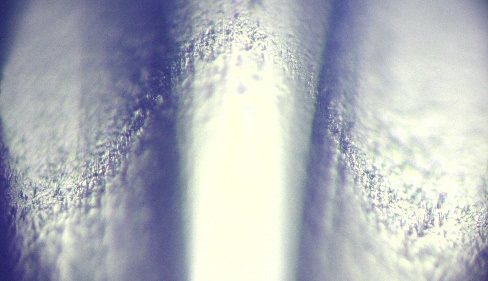
\includegraphics[width=1\linewidth]{cavity_unpolished}
  \end{minipage}
  \hfill
  \begin{minipage}[ht]{0.32\linewidth}\centering
    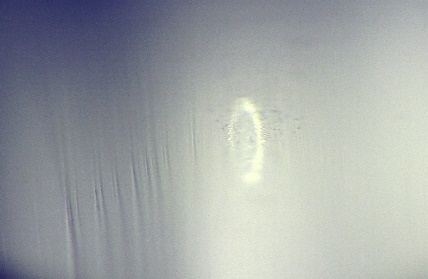
\includegraphics[width=1\linewidth]{cavity_polished_bad}
  \end{minipage}
  \hfill
  \begin{minipage}[ht]{0.32\linewidth}\centering
    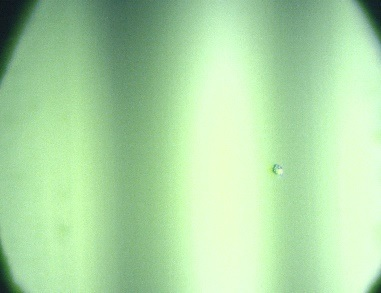
\includegraphics[width=1\linewidth]{cavity_polished_good}
  \end{minipage}
  \caption{Фрагмент поверхности резонатора с радиусом кривизны боковой поверхности 50 мкм (ширина выступа около 70 мкм). Слева сразу после точения изношенным резцом. Посередине фрагмент со сколом размером 20 на 50 мкм. Справа - после полировки алмазными суспензиями.}
  \label{cavity_polished}
\end{figure}

При увеличении глубины резки (depth of cut) до 6 мкм и более возможен хрупкий режим точения со сколами кристалла и повышенным износом резца. После очистки микрорезонатора проводится проверка качества получившейся поверхности в микроскоп для обнаружения возможных шероховатостей.

Так как обычный оптический микроскоп имеет дифракционный предел, дефекты малого размера в нем не видны, и на большом увеличении глубина резкости минимальна, видна очень малая область тороидальной боковой поверхности (не более 10-20 мкм), то контроль качества осуществлялся последовательным измерением добротности мод после полировки новыми алмазными суспензиями.

Дополнительно может быть произведен контроль качества боковой поверхности с помощью оптического профилометра Zygo NewView 7300. Результат измерения приведен на рис. \ref{cavity_profilometer}, измерены шероховатости размером 0.25 мкм.

\begin{figure}[ht]
\centering
  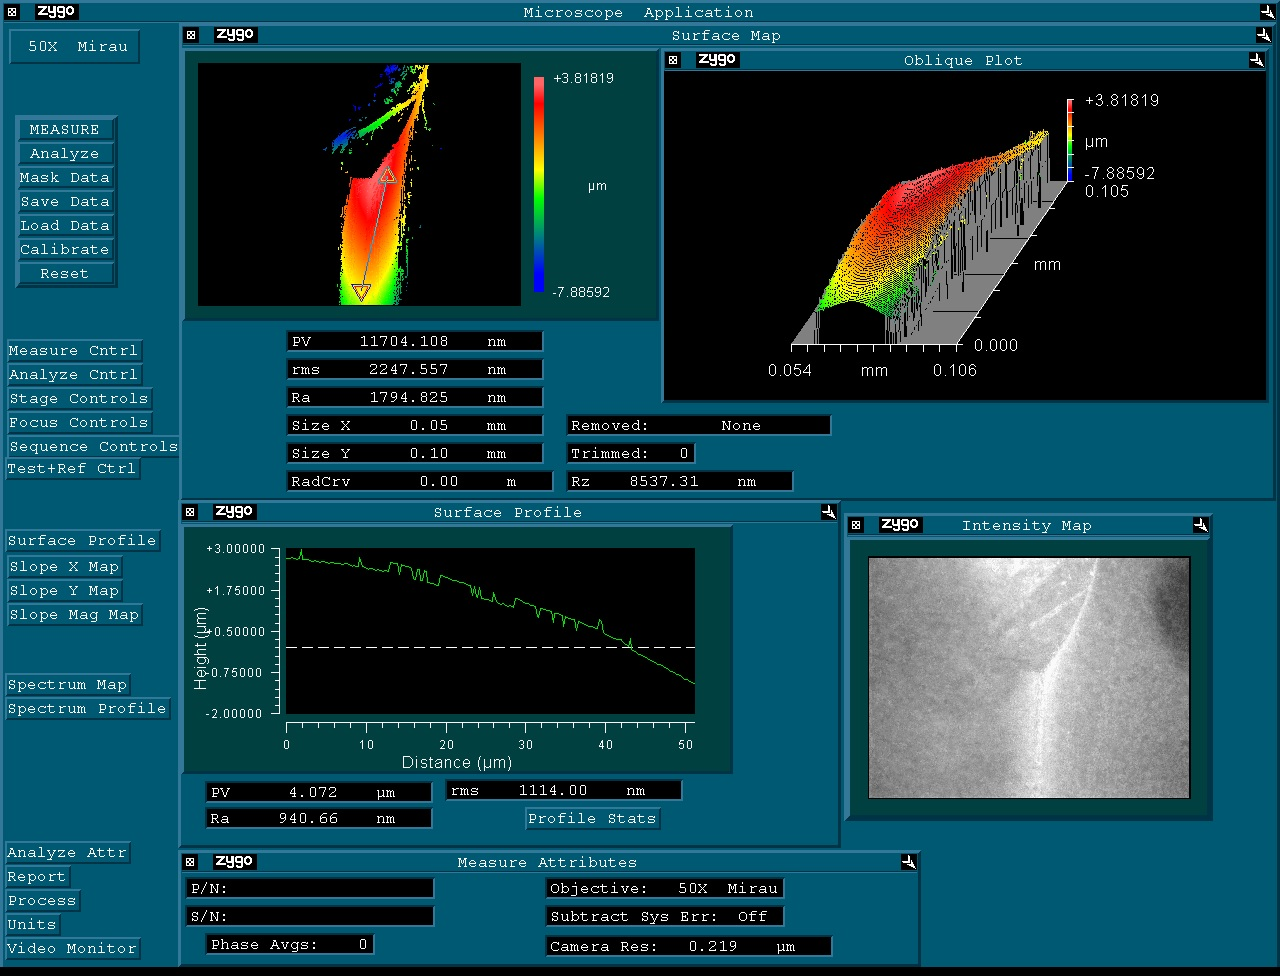
\includegraphics[width=0.5\linewidth]{cavity_profilometer}
  \caption{Измерение качества боковой поверхности с помощью оптического профилометра}
  \label{cavity_profilometer}
\end{figure}

Достаточным условием для оценки качества поверхности является проверка добротности после полировки. К сожалению, при таком способе оценки качества поверхности можно упустить технические ошибки, возникающие при полировке, т.к. в данном случае о качестве можно судить только по косвенному признаку – добротности. Измерение добротности производилась следующими методами: калибровка частоты дается боковыми линиями фазовой модуляции сканирующего лазера, зная частоту модуляции, можно аппроксимировать лоренцевскую форму резонанса МШГ. Для измерения ширины линии резонанса меньше 500 кГц лучше использовать метод звона, при котором либо быстро выключается, либо быстро перестраивается по частоте лазер накачки и проводится прямое измерение времени звона оптического резонатора по затухающему сигналу фотодетектора. Для измерения сверхвысоких добротностей необходимо использовать мощность лазера меньше 1 мВт, чтобы избежать нелинейных уширений.

В таблице \ref{table_turning_params} представлены параметры точения, при которых получались наилучшие результаты для различных материалов. 

\begin{table} [htbp]% Пример записи таблицы с номером, но без отображаемого наименования
	\centering
	\parbox{17cm}{% чтобы лучше смотрелось, подбирается самостоятельно
        %\captionsetup{format=tablenocaption}% должен стоять до самого caption
        \caption{Параметры алмазного точения резонаторов из различных кристаллических материалов}%
        \label{table_turning_params}%
    	\begin{tabular}{||c|c|c|c|c||}
\hline
\multicolumn{1}{|p{2cm}|}{\centering Материал} & \multicolumn{1}{|p{2cm}|}{\centering Скорость вращения шпинделя \\ обороты в мин} & \multicolumn{1}{|p{2cm}|}{\centering Скорость движения резца \\ мкм/оборот} & \multicolumn{1}{|p{2cm}|}{\centering Глубина захода резки \\ мкм} & \multicolumn{1}{|p{2cm}|}{\centering Охлаждающая \\ жидкость}\\
%Материал & Скорость вращения шпинделя, обороты в мин & Скорость движения резца, мкм/оборот & Глубина захода резки, мкм & Охлаждающая жидкость\\
\hline
$MgF_2$ & 400-1500 & 0.25-1 & 0.5-1 & да/нет \\
\hline
$BaF_2$ & 1000-2500 & 1-2.5 & 0.5-2 & нет \\
\hline
$CaF_2$ & 700-2500 & 1-2 & 1 & да/нет \\
\hline
$LiNbO_3$ & 900-1500 & 1-2.5 & 1-4 & нет \\
\hline
$LiTaO_3$ & 900 & 1-2 & 1-2 & нет \\
\hline
$Si$ & 500 & 1 & 0.5-1 & да \\
\hline
$TGG$ & 700 & 1 & 0.5-1 & нет \\
\hline
\end{tabular}

	}
\end{table}

\subsection{Практические замечания по изготовлению кристаллических микрорезонаторов}

Предобработка - раскол кристаллических пластин заготовок, при этом возможно образование напряжений внутри кусочков кристаллов. Мягкие материалы $BaF_2, CaF_2$ раскалываются на неконтролируемые куски при любой толщине заготовки. Распил алмазной пилой позволяет этого избежать. Однако для заготовок толщиной 100-200 мкм возможны внутренние трещины из-за неровности наклейки на подставку для распила. Необходимо использовать тонкие диски пилы с алмазным напылением. Выпиливание цилиндрических заготовок трубчатым сверлом малоэффективно, т.к. большая часть материала уходит в стружку и из-за больших биений сверла вероятно появление больших сколов.

Дизайн подставки \ref{cavity_scheme_big} диктуется размером цанги станка и удобством крепления в экспериментальных установках. Материал подставки латунь выбран из-за достаточно высокой теплопроводности для улучшения активной термостабилизации. Все кристаллические материалы для генерации оптических гребенок имели z-cut, т.ч. оптическая ось z совпадала с осью цилиндра.

Отжиг кристаллов для устранения внутренних дефектов проводился, но без прямого измерения улучшения добротности до и после, т.к. клей не позволяет нагревать до 700-800С наклееный на подставку резонатор, а в случае переклейки резонатора вероятность загрязнения велика и будет требоваться новая переполировка. При попытке отжига наклеенного резонатора из $BaF_2$ при 400С в кристалле возникло большое количество внутренних трещин.

Алмазное точение SPDT возможно в широком диапазоне параметров при использовании нового неизношенного резца. Качество поверхности фторида магния при этом высокое, т.ч. добротность резонатора может достигать $10^6$ (пример выступа резонатора с такой добротностью дан на рис. \ref{protrusion_unpolished}), что соответствует типичным значениям добротности в интегральных оптических резонаторах.

\begin{figure}[ht]
\centering
  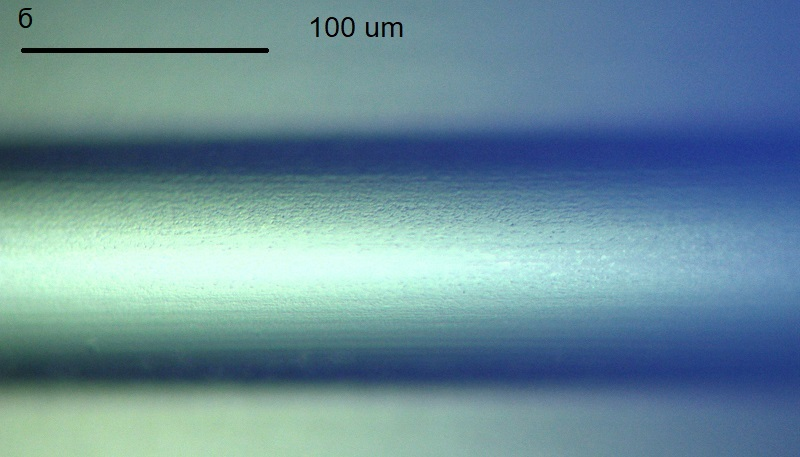
\includegraphics[width=0.5\linewidth]{protrusion_unpolished}
  \caption{Фотография поверхности резонатора из $MgF_2$ сразу после точения, в котором достигается добротность $10^6$ на 1550 нм.}
  \label{protrusion_unpolished}
\end{figure}

Основной недостаток метода алмазного точения - быстрый износ алмазного резца. На практике износ резца наступает за 100 м точения, что соответствует изготовлению 3 резонаторов. Далее качество получаемой поверхности заметно ухудшается и никакими более щадящими параметрами точения улучшить его нельзя. Изношенным резцом возможно точение твердых материалов $MgF_2$, но более мягкие $BaF_2, LiF$ могут давать сколы размерами в несколько сот микрон, недоступными для устранения полировкой \ref{cavity_damage}. Наиболее практично использовать для изготовления цилиндров заданного диаметра изношенный резец, а далее снимать финальный слой толщиной 10 мкм с помощью чистового неизношенного резца. Важно при этом регулярно проводить перекалибровку относительного положения изношенного и чистового резцов, т.к. сколы края алмаза могут достигать 10 мкм \ref{tool_damage}.

\begin{figure}[ht]
  \begin{minipage}[ht]{0.49\linewidth}\centering
    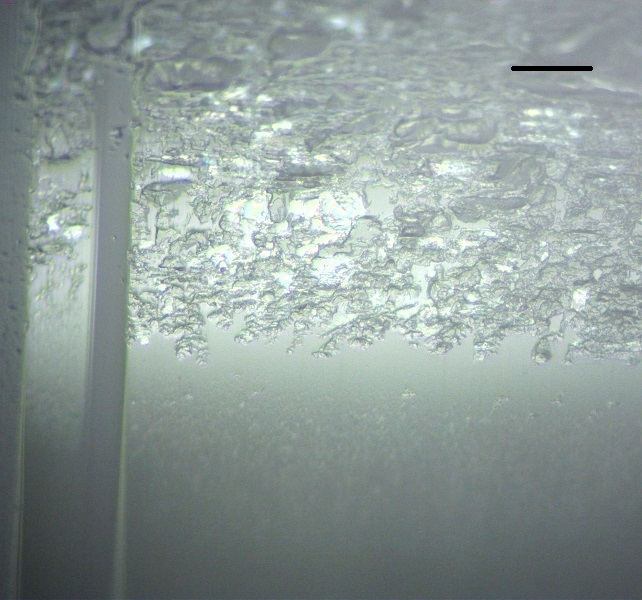
\includegraphics[width=1\linewidth]{cavity_damage}
  \end{minipage}
  \hfill
  \begin{minipage}[ht]{0.49\linewidth}\centering
    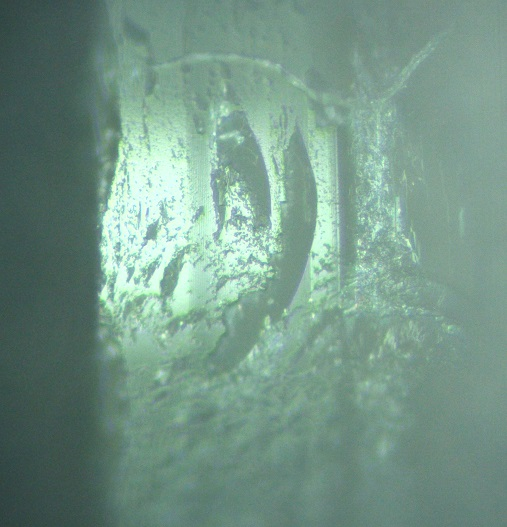
\includegraphics[width=1\linewidth]{cavity_damage_baf2}
  \end{minipage}
  \caption{Слева фрагмент поверхности резонатора из $MgF_2$ после точения при неоптимальных параметрах, видны секторы хорошего и плохого качества поверхности, соответствующие точению различных кристаллических срезов, такие дефекты можно убрать полировкой без сохранения геометрии резонатора. Справа фрагмент поверхности резонатора из $BaF_2$ после точения изношенным резцом, видны глубокие сколы, которые нельзя убрать полировкой.}
  \label{cavity_damage}
\end{figure}

\begin{figure}[ht]
\centering
  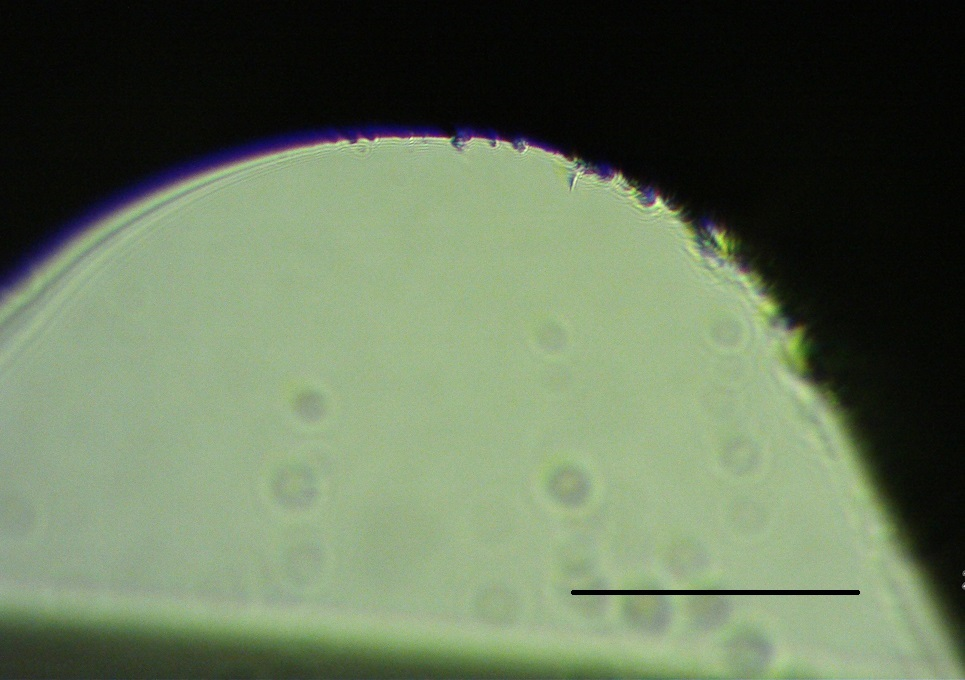
\includegraphics[width=0.5\linewidth]{tool_damage}
  \caption{Рабочий край изношенного алмазного резца с радиусом кривизны 500 мкм, видны сколы по краю характерным размером 10 мкм. При дальнейшем использовании резца возможно образование скола алмаза по прямой линии, таким резцом можно грубо вытачивать цилиндры заданного диаметра.}
  \label{tool_damage}
\end{figure}

В литературе по точению основными методами борьбы с износом являются более щадящие параметры точения (уменьшение глубины резки и действующей силы, пропорциональной скорости вращения) и использовании охлаждающей жидкости. Важно понимать, что при использовании охлаждающей жидкости меняется режим точения и следует заново подбирать оптимальные параметры. Уменьшение же глубины резки приводит к пропорциональному росту времени точения. Охлаждающая жидкость при изготовлении большинства резонаторов из $MgF_2$ не применялась, т.к. нет удобной системы вентиляции, и ее расход велик, т.ч. бака может не хватать на типичное точение в 6-10 часов, также заводская жидкость содержала маслянистые фракции, которые могут повредить шпиндель на воздушных подшипниках.

Полировка при хорошей центровке микрорезонатора возможна не только последовательным уменьшением зерна суспензии, но и при грубой полировке зерном 2.5-4 мкм для удалений сколов с характерными размерами 5-15 мкм, далее зерном 0.5 мкм и сразу 0.1 мкм для финальной полировки. Стандартное правило - удаление материала в 3-4 кратном размере диаметра зерна. Таким способом повторяемо достигается добротность $5*10^8$ на длине волны $1550 нм$ в кристаллах $MgF_2$ из заготовки VUV качества материала \ref{ringdown}.

\begin{figure}[ht]
\centering
  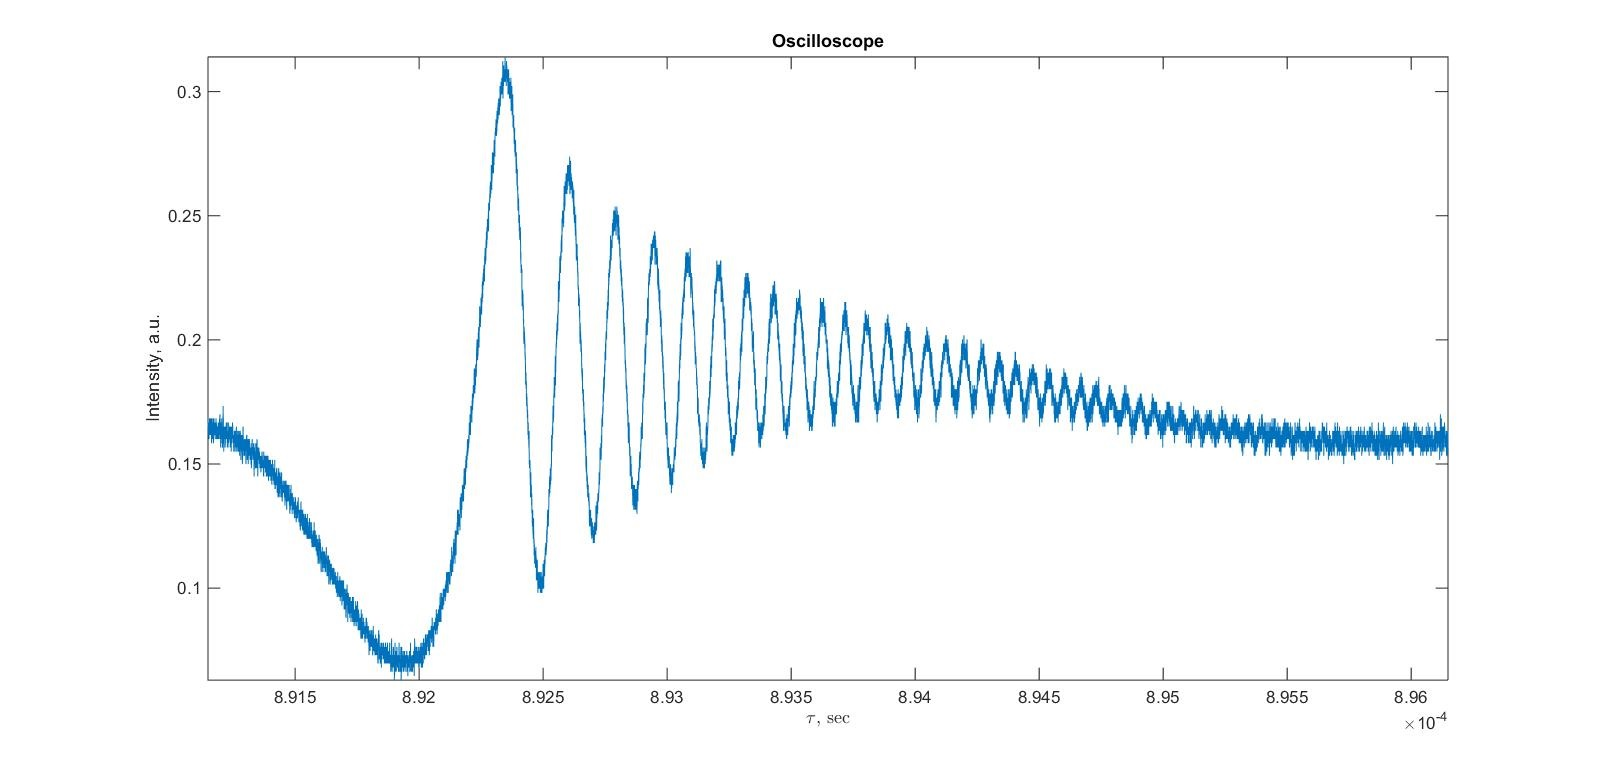
\includegraphics[width=0.5\linewidth]{ringdown}
  \caption{Определение добротности резонатора из $MgF_2$ прямым измерением времени звона. Соответствующее значение добротности $2*10^9$}
  \label{ringdown}
\end{figure}


Изготовление прямоугольных микровыступов даже новыми острыми резцами не удалось для диаметров резонатора больше 4 мкм для $MgF_2$ и получилось для диаметров около 1 мм \ref{protrsuion_rect}. Этот резонатор далее детально не изучался.

\begin{figure}[ht]
\centering
  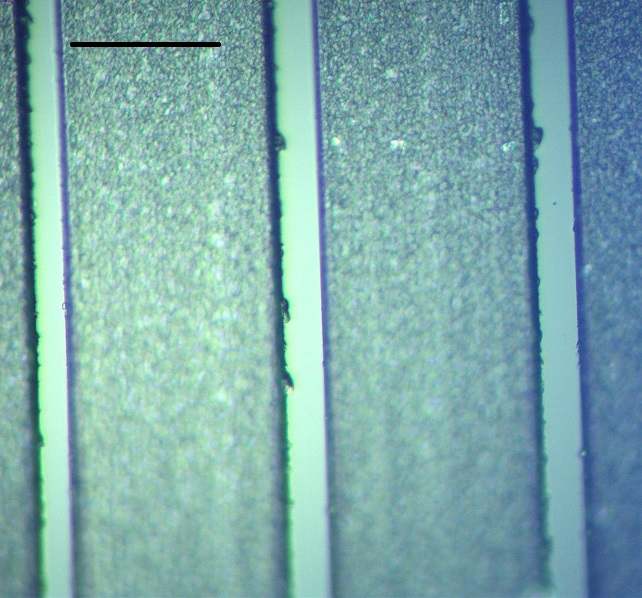
\includegraphics[width=0.5\linewidth]{protrsuion_rect}
  \caption{Фрагмент поверхности резонатора с прямоугольными выступами размером 5 на 15, 20, 25 мкм для контроля ДГС резонатора. Показано качество поверхности до полировки, видны сколы по 5 мкм на выступе из-за износа острого резца.}
  \label{protrsuion_rect}
\end{figure}

\section{Экспериментальное наблюдение оптических частотных гребенок и солитонов в резонаторах из $MgF_2$}


\subsection{Экспериментальная установка и результаты генерации солитонов}

\begin{figure}[ht]
\centering
  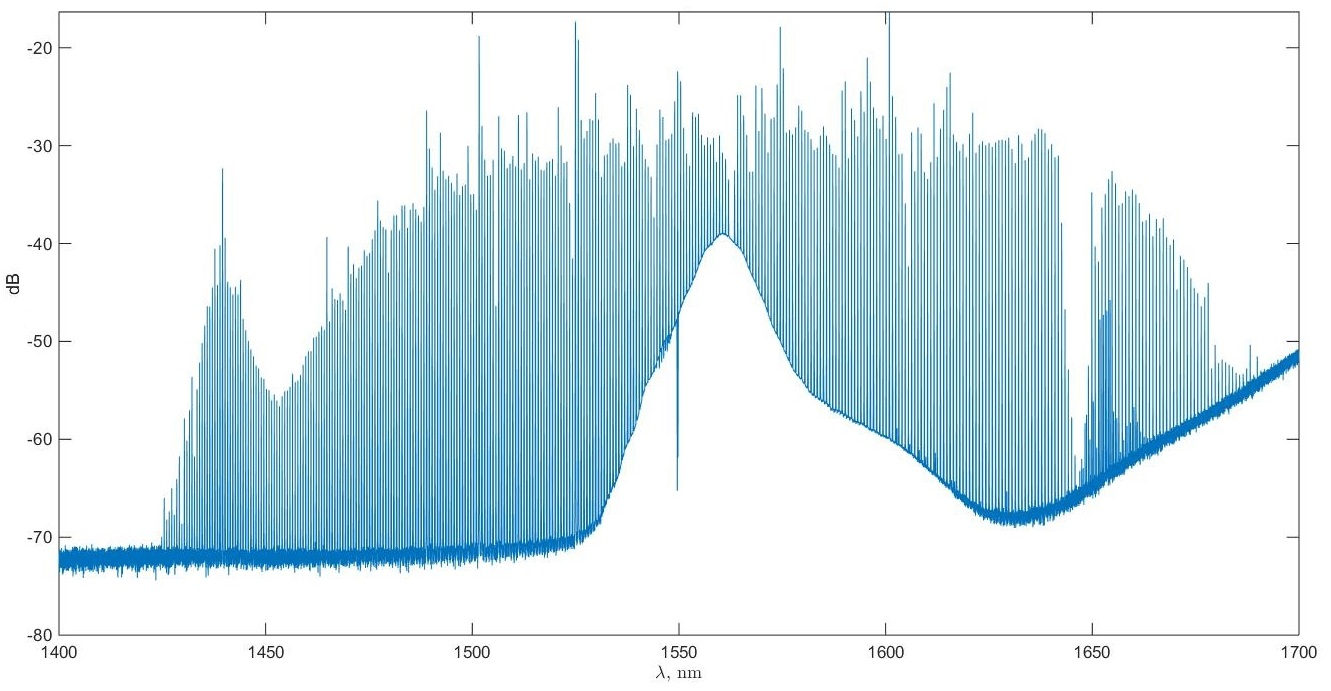
\includegraphics[width=0.4\linewidth]{wide_comb_93GHz}
  \caption{Оптический спектр широкой оптической гребенки в шумном режиме с ОСД около 93 ГГц, полученный в резонаторе диаметром 0.75 мм и радиусом кривизны 150 мкм.}
  \label{wide_comb_93GHz}
\end{figure}


\begin{figure}[ht]
  \begin{minipage}[ht]{0.49\linewidth}\centering
    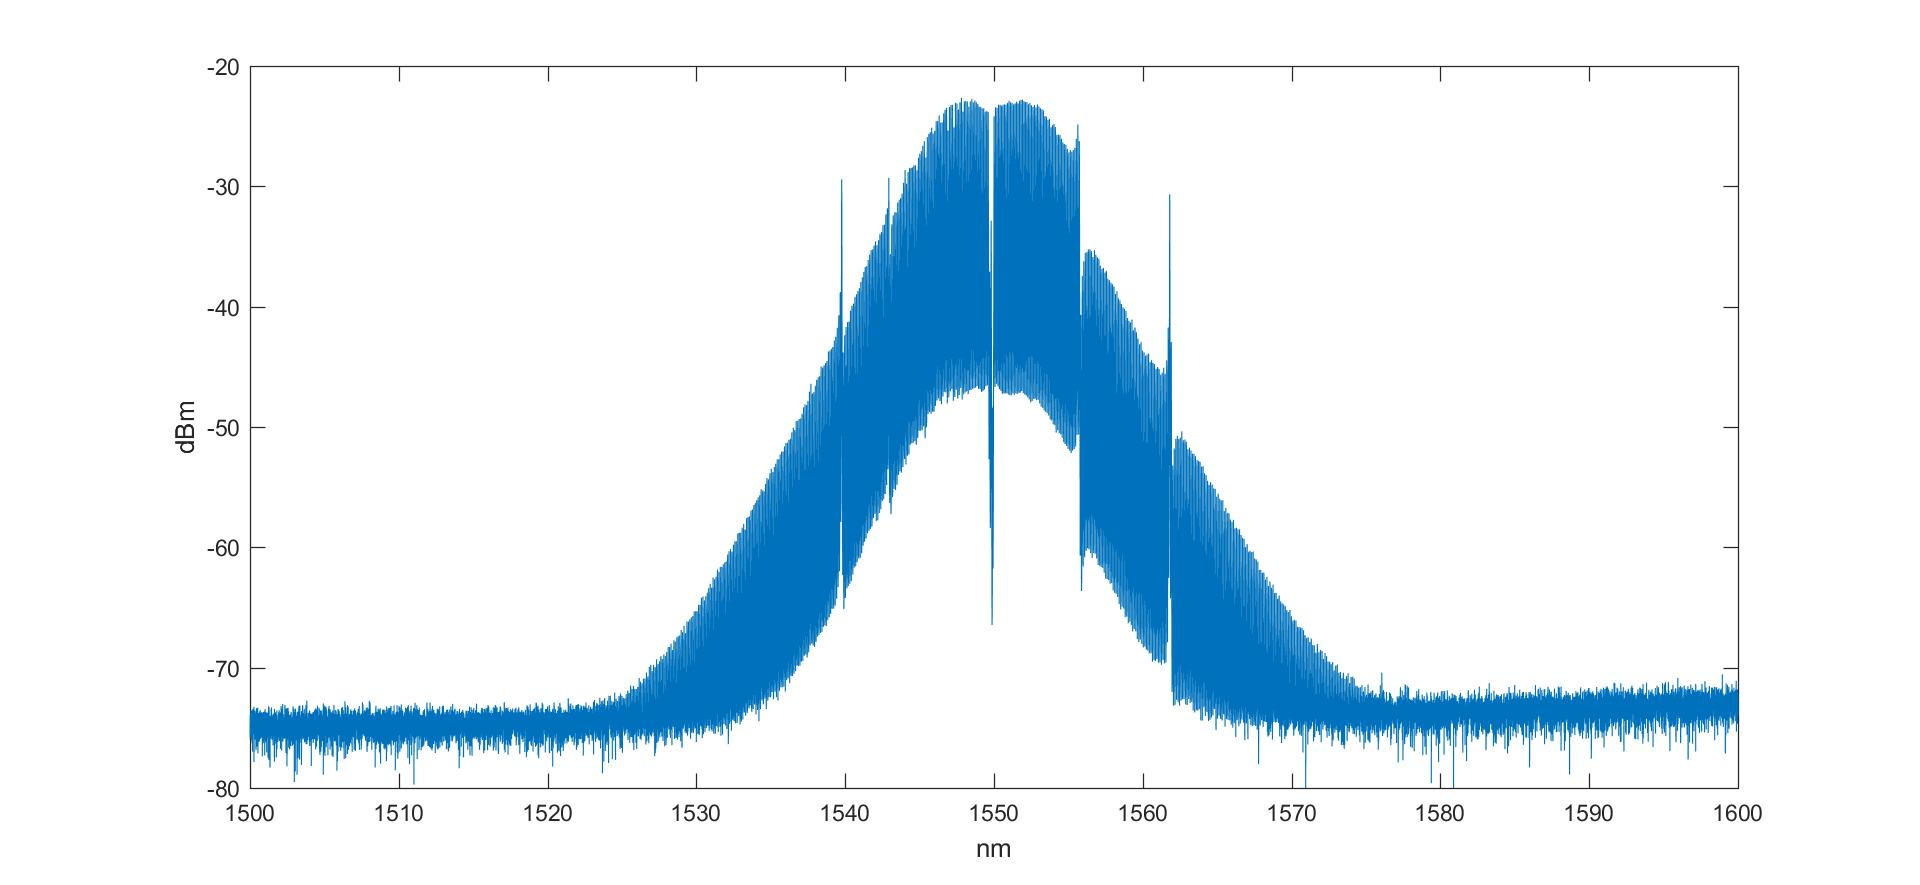
\includegraphics[width=1\linewidth]{noisy12}
  \end{minipage}
  \hfill
  \begin{minipage}[ht]{0.49\linewidth}\centering
    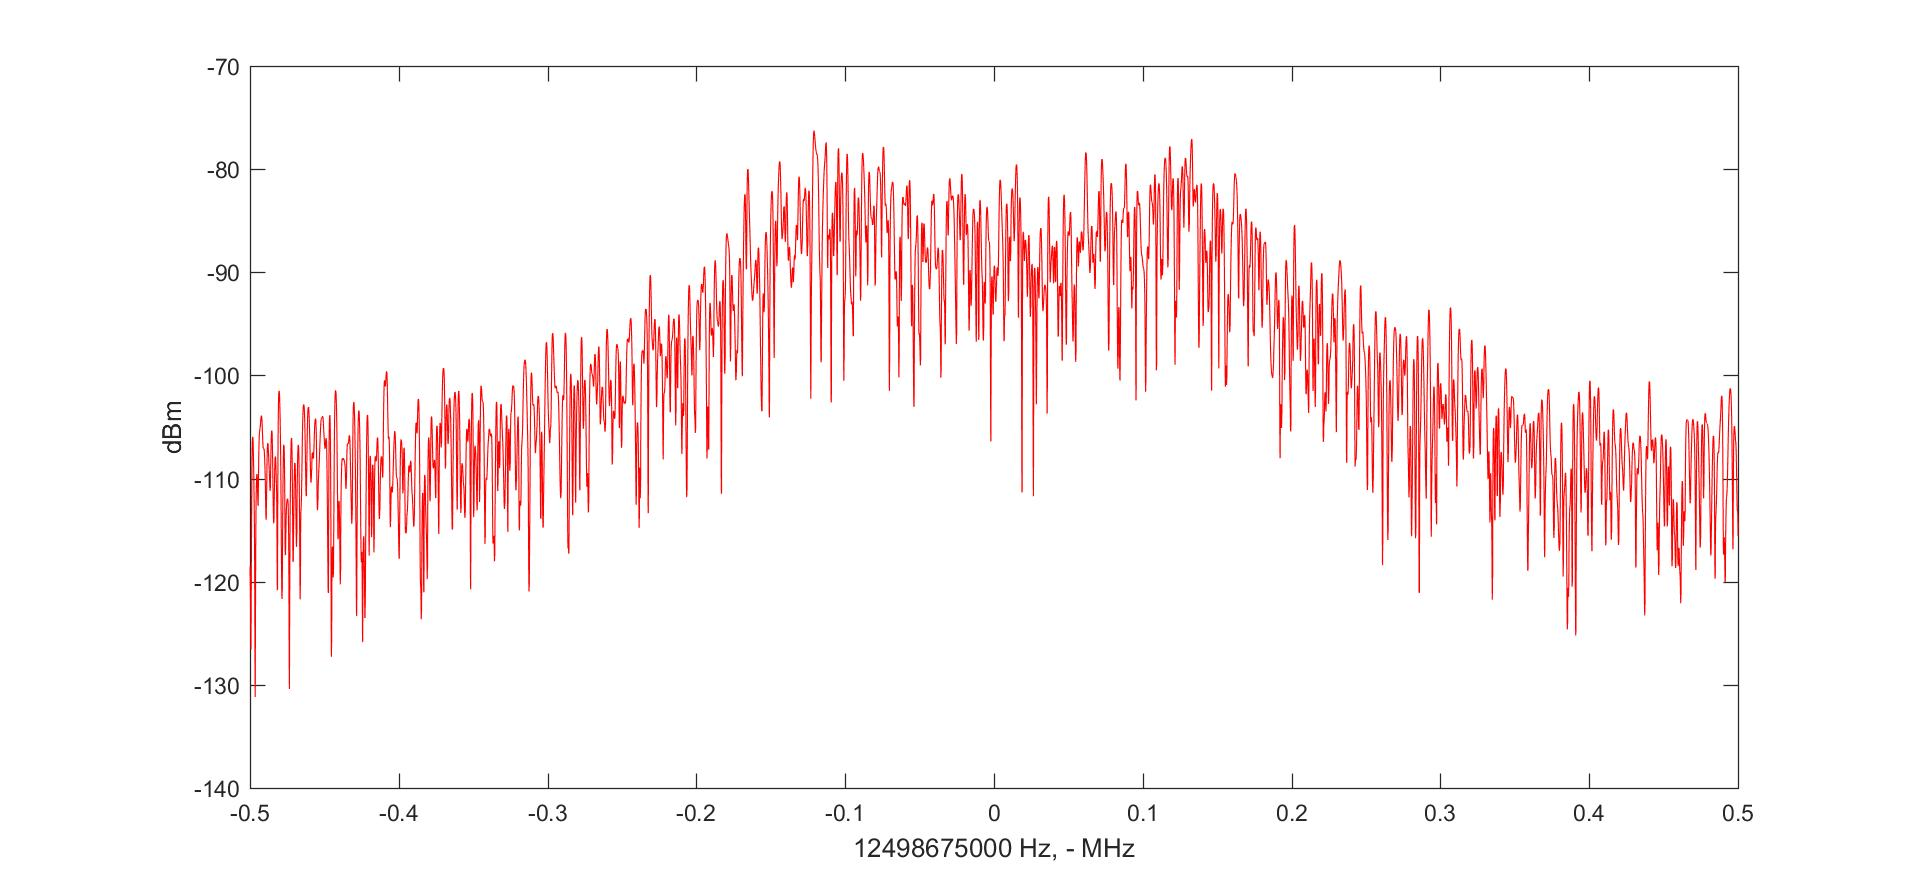
\includegraphics[width=1\linewidth]{noisy12_beatnote.jpg}
  \end{minipage}
  \caption{Слева оптический спектр оптической гребенки в шумном режиме. Справа соответствующий сигнал биений на частоте ОСД 12.48 ГГц.}
  \label{lathe}
\end{figure}

\begin{figure}[ht]
  \begin{minipage}[ht]{0.49\linewidth}\centering
    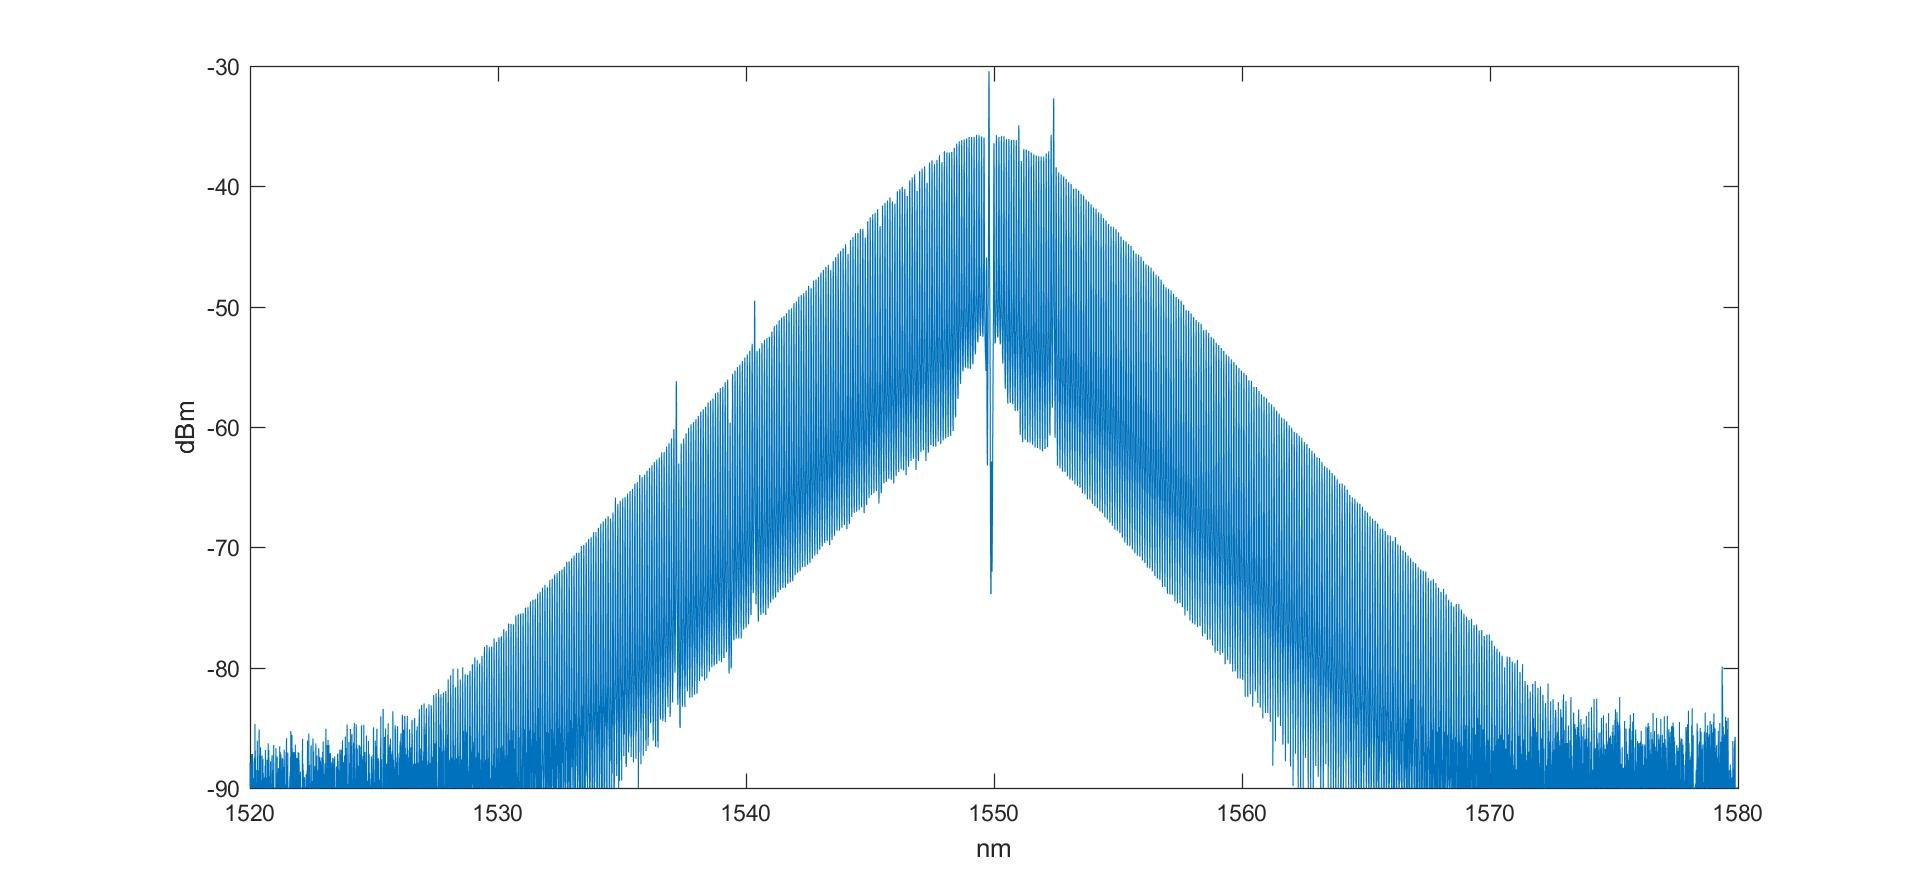
\includegraphics[width=1\linewidth]{soliton_12GHz}
  \end{minipage}
  \hfill
  \begin{minipage}[ht]{0.49\linewidth}\centering
    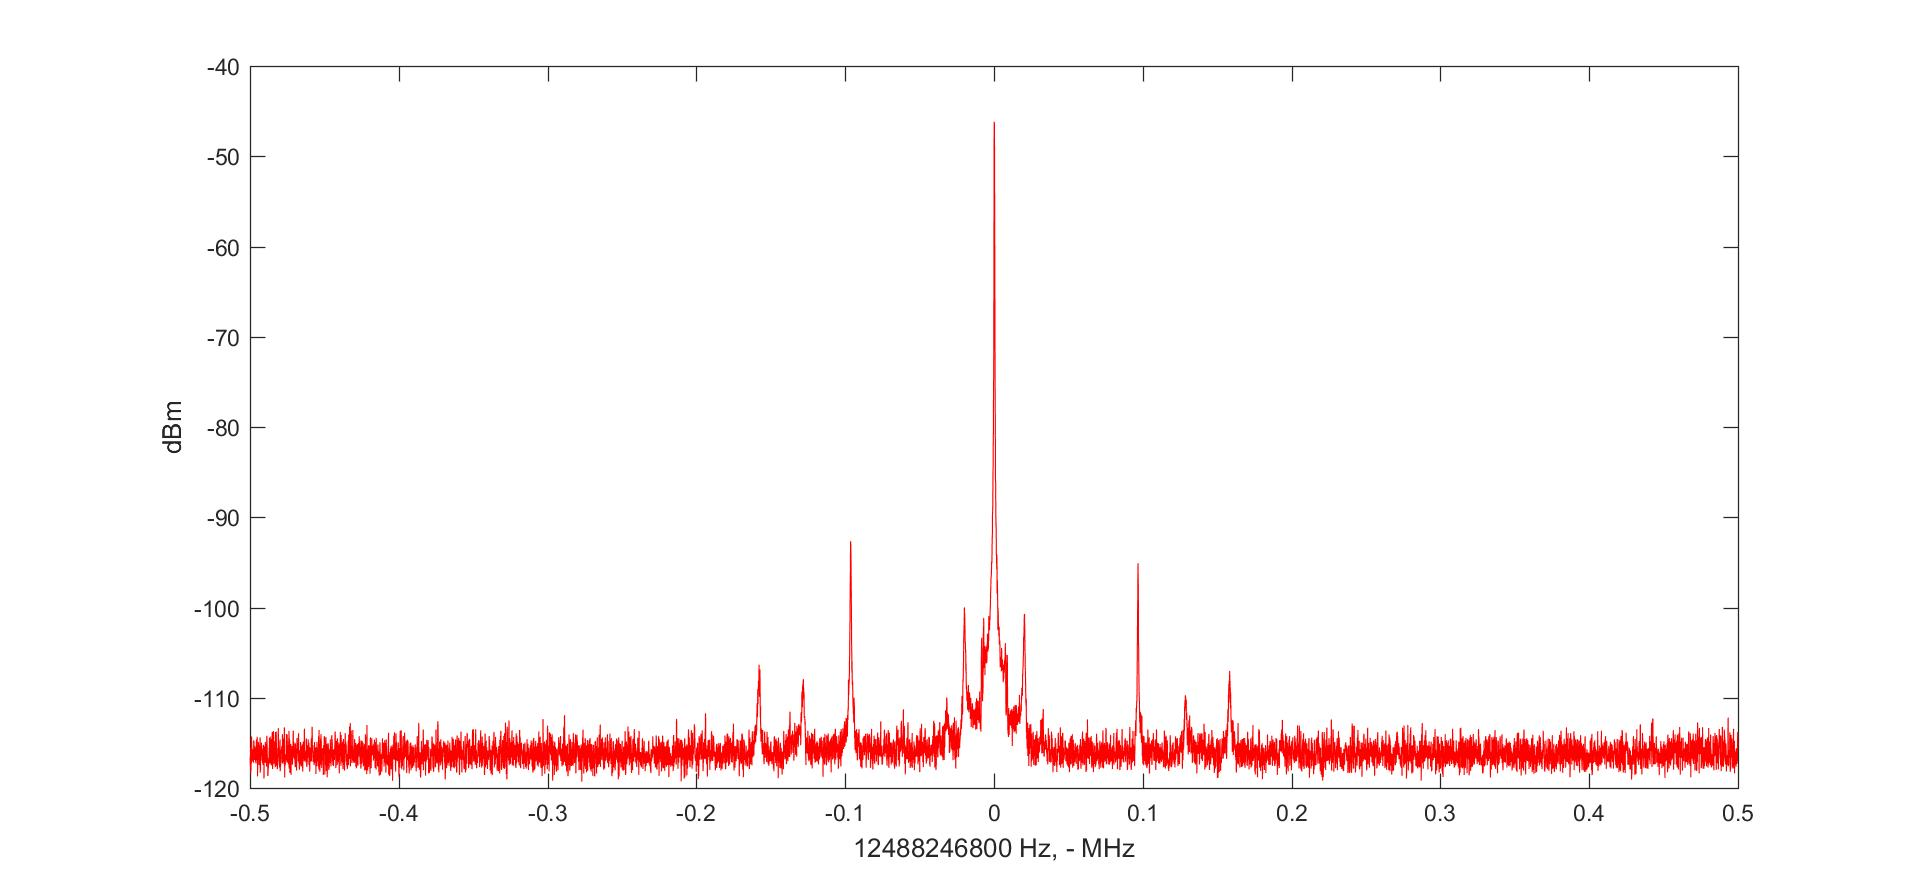
\includegraphics[width=1\linewidth]{soliton12_beatnote.jpg}
  \end{minipage}
  \caption{Слева оптический спектр оптической гребенки в односолитонном режиме. Справа соответствующий узкий сигнал биений на частоте повторения солитона 12.48 ГГц}
  \label{lathe}
\end{figure}


\begin{figure}[ht]
\centering
  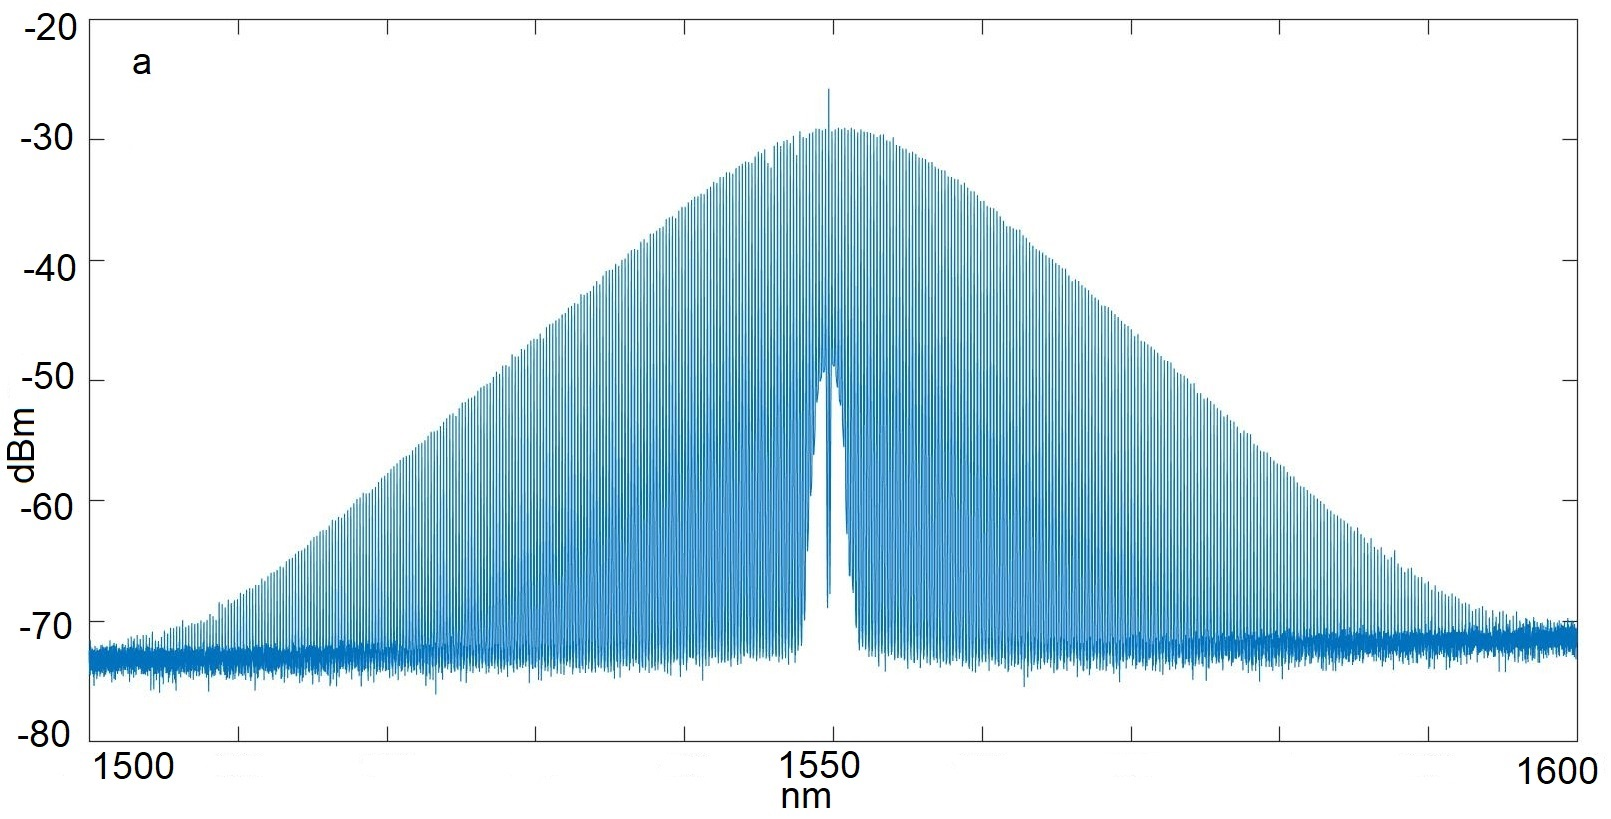
\includegraphics[width=0.5\linewidth]{clean_27GHz_single_soliton}
  \caption{Оптический спектр односолитонного режима с ОСД около 27 ГГц, полученный в резонаторе диаметром 2.4 мм и радиусом кривизны 80 мкм. Регулируя положение элемента связи (оптического волокна) с резонатором возможно добиться спектра с минимальным количеством пересечений мод}
  \label{clean_27GHz_single_soliton}
\end{figure}


%\subsection{Методы контроля и стабилизации частоты и отстройки лазера накачки}
%метод VNA, обзор работы Карпова, картинка RIGOL

%более удобный метод PDH, минуc - нет возможности менять отстройку

%\subsection{Метод стабилизации частоты повторения солитонов с помощью амплитудной модуляции лазера накачки}
%амплитудная модуляция на кратных фср частотах приводит к узкой области захватывания частоты повторения солитонов

\subsection{Методы достижения односолитонного режима}

В литературе было предложено несколько методом детерминированного достижения односолитонного режима в оптических микрорезонаторах. Первый метод предполагает одновременную перестройку частоты лазера накачки и изменение его мощности для избежания хаотического режима гребенки \cite{Jaramillo2015}. Другим способом является не перестройка частоты лазера, а сдвиг частоты резонанса МШГ путем изменения его температуры \cite{Joshi2016} или контроля времени жизни свободных носителей (для интегральных резонаторов) \cite{Yu2016}.

Рассмотрим случай \cite{Lobanov2016} фазовой $f(t)=F e^{i\varepsilon\sin\Omega t}$ и амплитудной $f(t)=F(1+\varepsilon\cos\Omega t)$  модуляции с частотой $\Omega$ и глубиной модуляции $\varepsilon$. Моделировалась система нелинейных связанных уравнений \ref{set_am}. Тепловые эффекты не рассматривались. В численных симуляциях не рассматривались частотныя зависимость нелинейности, потерь и пересечения мод, взаимодействия между мод. Предполагая, что частота модуляции близка к ОСД резонатора:
 
\begin{equation}
\frac{\partial a_\mu}{\partial \tau}=-(1+\zeta_\mu)a_\mu+i\sum_{\mu',\mu^{''}}a_{\mu^{'}} a_{\mu^{''}} a^{*}_{\mu^{'}+\mu^{''}-\mu}+f_{\mu}\exp(i\mu\Delta\tau).
\end{equation}

Где обозначения соответствуют принятым в этой работе и $f_\mu=F J_\mu(\varepsilon)$ для фазовой модуляции и $f_{-1,0,1}=F[\varepsilon/2,1,\varepsilon/2]$,  $f_{\mu \neq -1,0,1}=0$ для амплитудной модуляции и безразмерной величине накачки $F$. $J_\mu(\varepsilon)$ функция Бесселя порядка $\mu$, $\Delta=2(D_1-\Omega)/\kappa$ нормализованная отстройка от точного значения ОСД, $D_1$ соответствует $2\pi\times$FSR. Все номера мод $\mu$ определены относительно 0 моды накачки. Дисперсионный закон дается разложением $\omega_\mu=\omega_0+D_1\mu+\frac{1}{2}D_2\mu^2+...$ и пренебрегая дисперсией третьего и более высоких порядков, получаем выражение для нормализованной отстройки: $\zeta_\mu=2(\omega_0-\omega_p)/\kappa+(D_2/\kappa)\mu^2$. $D_2>0$ соответствует аномальной дисперсии. Моделировалось 525 мод. Для анализа вычислялась средняя мощность внутри резонатора $U=\sum_{\mu} \vert a_\mu\vert^2$ для разных занчений нормализованной отстройки $\zeta_0$ и соответствующий профиль поля в микрорезонаторе $\psi(\varphi)=\sum_{\mu} a_{\mu}\exp(i\mu\varphi)$.

Для возбуждения солитонов лазер накачки перестраивается линейно по частоте $\zeta_{0}(\tau)=\zeta_{0}(0)+\alpha\tau$ от эффективной синей отстройки $\zeta_0(0)<0$, через нулевую отстройку в эффективную красную область $\zeta_0\gg0$ для сканирования всей области существования солитона. Формирование солитонов дает характерные ступеньки в генерируемом свете. Если перестройку лазера остановить на частоте, лежащей на ступеньке, то солитонное состояние является стабильным во времени. Максимальная частота отстройки области существования солитона \cite{Herr2014} дается $\zeta_{0\text{max}}\sim {\pi^2 F^2}/{8}$. В симуляциях использовались следующие значения $F\approx 4.11$, $D_{2}/\kappa\approx {0.01}$ и $\zeta_{0\text{max}}\approx 20.8$

Для набора статистики проводилось по 100 симуляций для каждого набора параметров и строилось распределение вероятности количества генерируемых солитонов. Известно \cite{Herr2014, Karpov2016}, что в случае немодулированной накачки ($\varepsilon=0$) количество возбуждаемых солитонов может варьироваться от скана к скану. Это подтверждается и при численном моделировании рис. \ref{Mod4}(a)-\ref{Mod4}(b). Среднее количество возбуждаемых солитонов увеличивается с увеличением мощности накачки и уменьшении ДГС резонатора. При уменьшении скорости сканирования лазера более вероятными становятся малосолитонные режимы.

\begin{figure}[ht]
\centering
  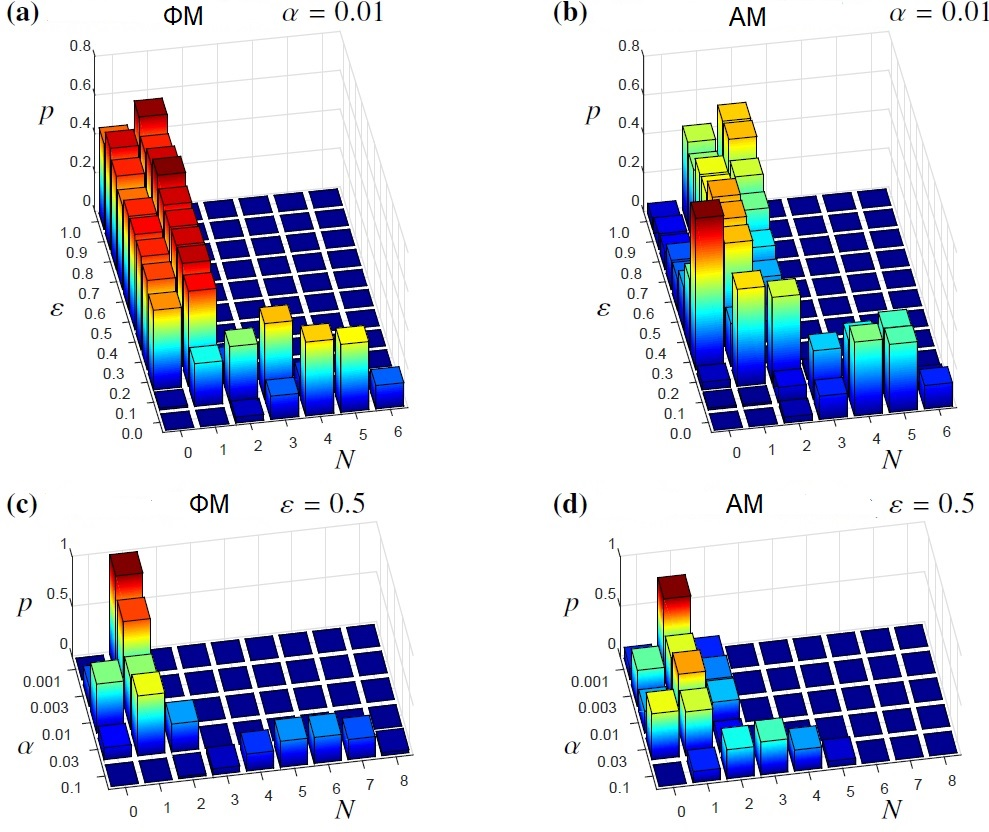
\includegraphics[width=0.85\linewidth]{Modulation4_s}
  \caption{Распределение вероятностей количества возбужденных солитонов от глубины модуляции $\varepsilon$ и скорости сканирования $\alpha$. Конечная отстройка $\zeta_0=18$ для фазовой и $\zeta_0=15$ для амплитудной модуляции. В обоих случаях $F\approx 4.11$ и $100$ реализациях.}
  \label{Mod4}
\end{figure}

Статистика значительно изменяется при включении слабой резонансной модуляции ($\Delta=0$) на частоте 1 ОСД. Как показано на рис. \ref{Mod4}(a)-\ref{Mod4}(b), если глубина модуляции достаточно высокая ($\varepsilon> 0.2$), то более вероятными становятся состояния с меньшим количеством солитонов. Для фазовой модуляции возможны два равновероятных сценария - возбуждение односолитонного режима или отсутствие генерации солитонов вообще. Для амлитудной модуляции наиболее вероятные сценарии одно- или двухсолитонные состояния. Этот факт может быть объяснен взаимодействием солитонов: под действием фазовой модуляции солитоны внутри микрорезонатора двигаются к положению равновесия. Два солитона сталкиваются и уничтожаются, т.ч. суммарное число солитонов уменьшается на 2. Либо два солиотна сливаются в один с уменьшением общего числа на 1.

Важным фактором увеличивающем вероятность односолитонного режима является уменьшение скорости сканирования частоты лазера. При малых $\alpha$ для детерминированного достижения односолитонного режима требуется меньшая глубина модуляции. После остановки перестройки частоты лазера и достижения солитонного режима, возможно отключение модуляции с сохранением солитона, если глубина модуляции невелика.

При модуляции не строго на частотое 1 ОСД (Рис. \ref{Detuned}), а с неточностью $\Delta$, вероятность достижения односолитонного режима ниже и предложенный метод не так эффективен, что частично можно компенсировать увеличением глубины модуляции.

\begin{figure}[ht]
\centering
  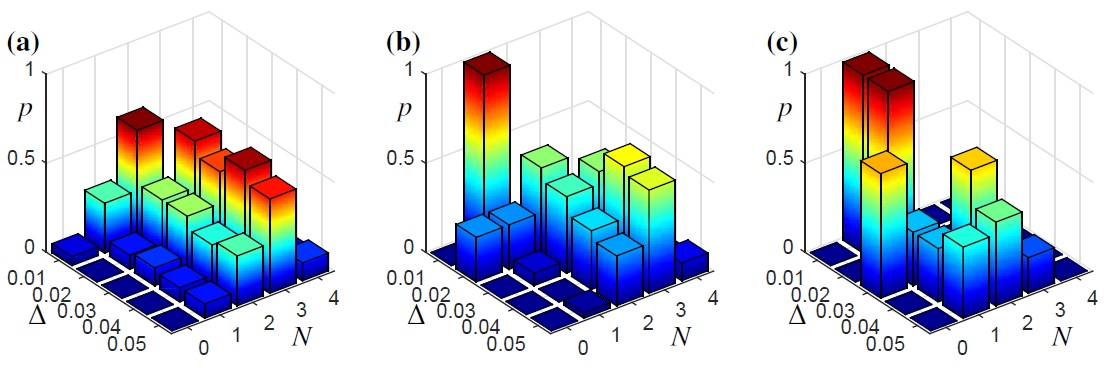
\includegraphics[width=0.85\linewidth]{detuned}
  \caption{Распределение вероятностей количества возбужденных солитонов при фазовой модуляции для различных значений неточности $ \Delta$  и $\varepsilon$  at  $\alpha=0.001$, $\frac{D_2}{\kappa}\approx 0.01 $. Конечная отстройка $\zeta_0=18$: (a) $\varepsilon=0.3$; (b) $\varepsilon=0.6$; (c) $\varepsilon=1.0$.}
  \label{Detuned}
\end{figure}

Для подтверждения численных симуляций был проведен эксперимент с резонатором из $MgF_2$. Резонатор имел диаметр 5.6 мм, радиус кривизны 35 мкм. Нагруженная ширина линии составила 500 кГц. Экспериментальная установка представлена на рис. \ref{chaos_order_experiment}(a).

\begin{figure}[ht]
\centering
  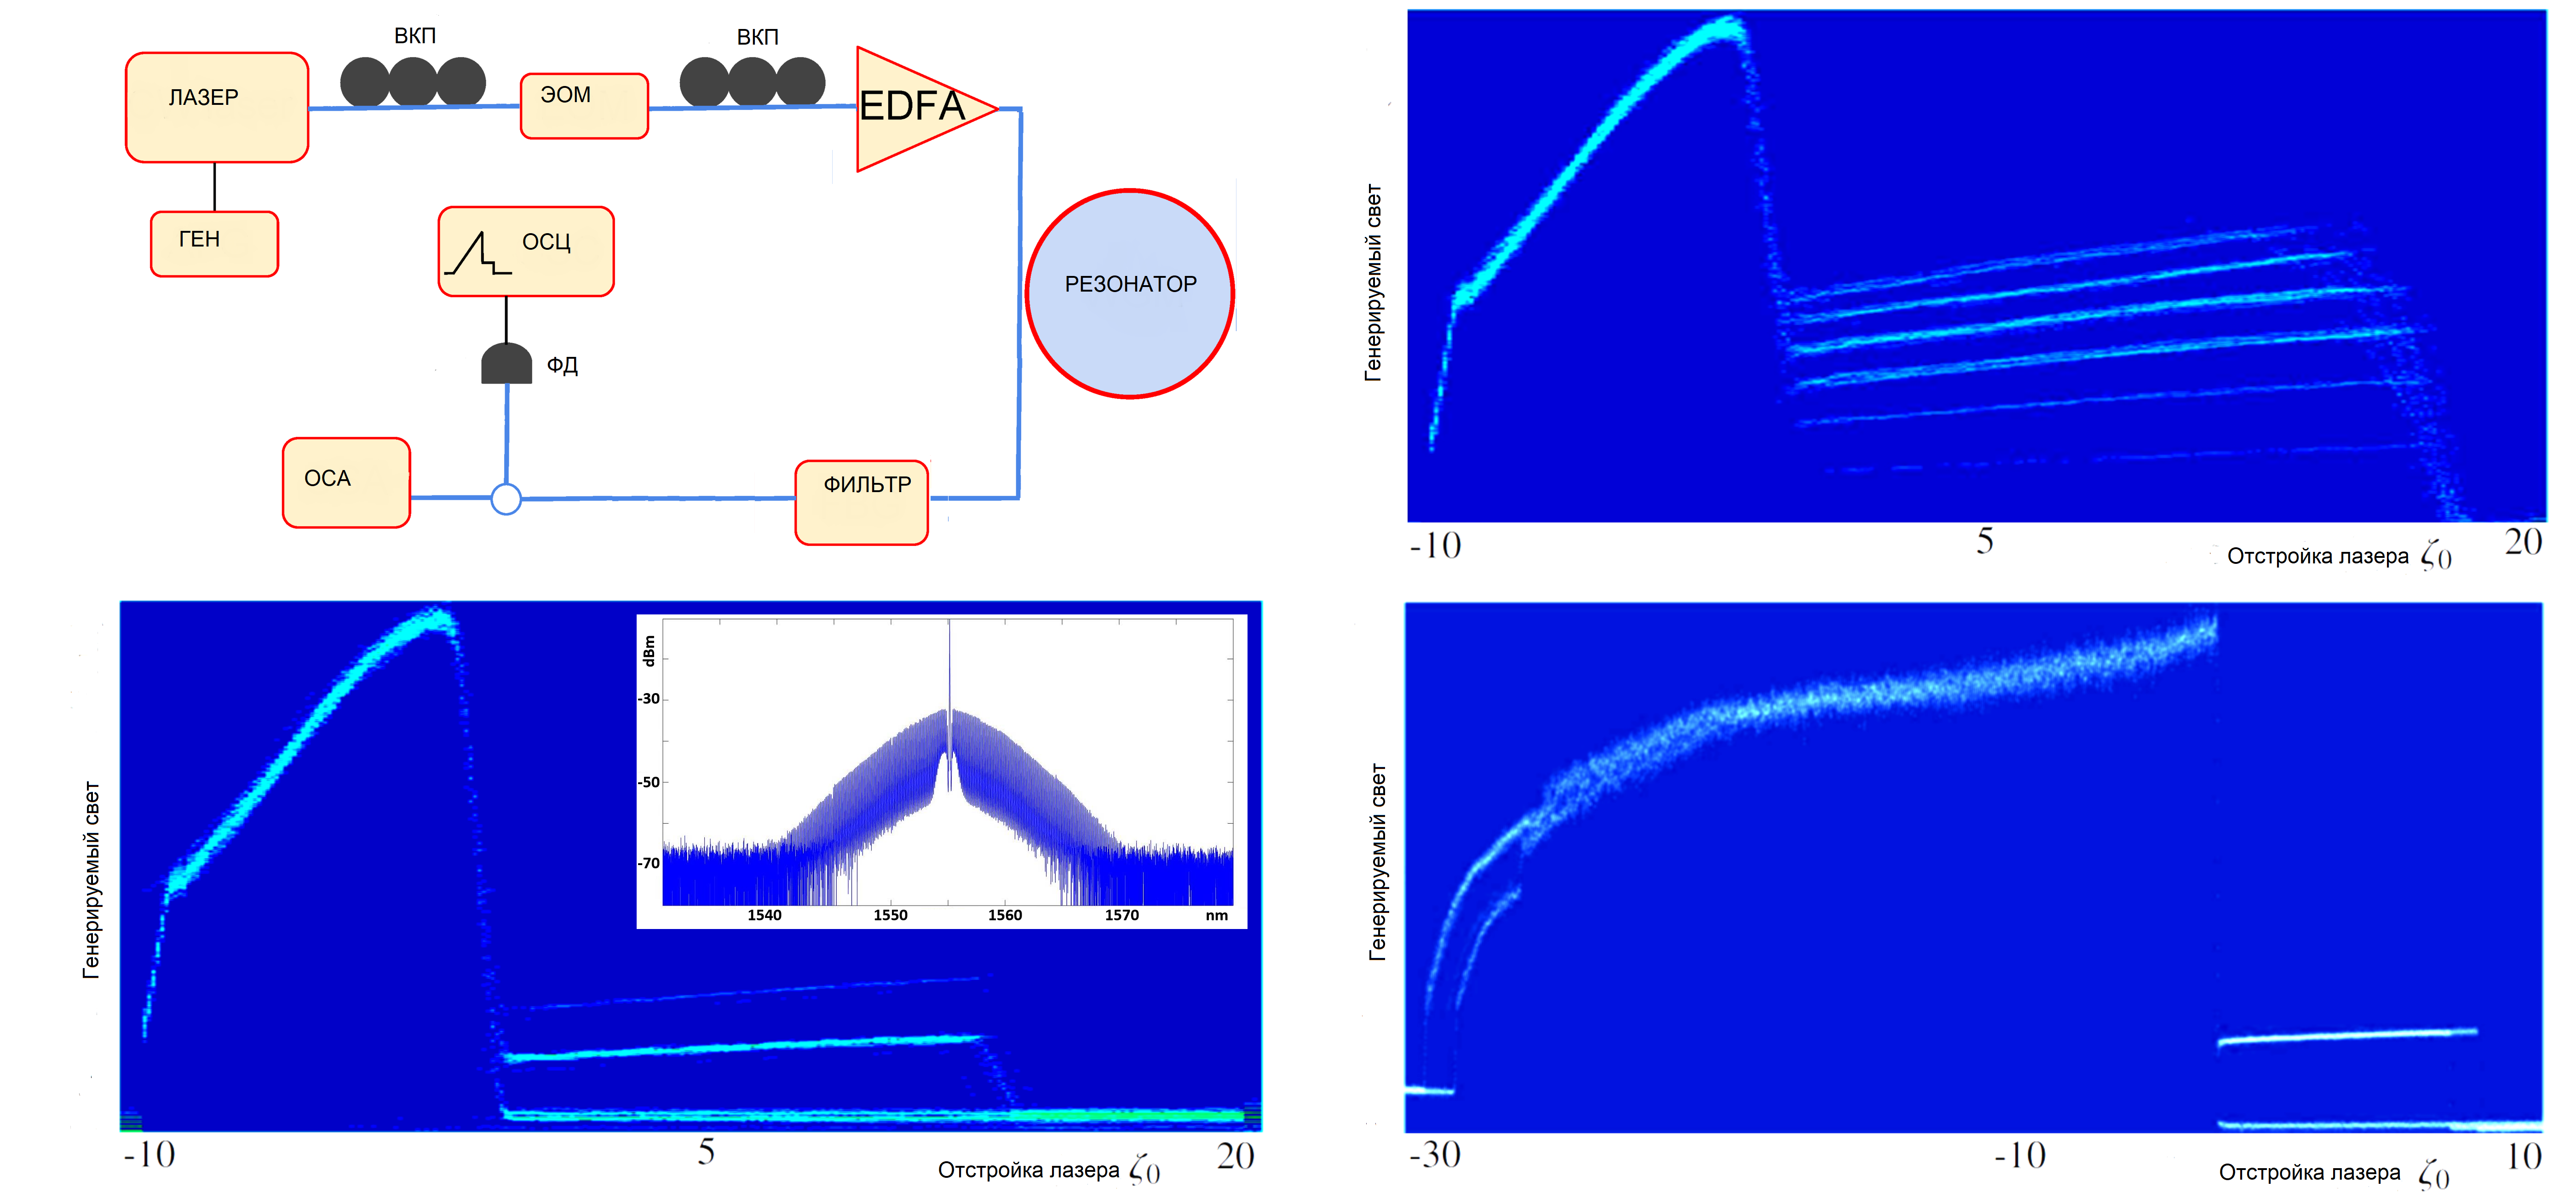
\includegraphics[width=1\linewidth]{Experiment_s}
  \caption{Экспериментальное измерение формирования солитонов при фазовой модуляции накачки и сканировании лазера. (a) экспериментальная установка (AFG, генератор сигналов произвольной формы; CW laser, узкополосный перестраиваемый лазер непрерывной мощности; FPC, волоконный контроллер поляризации, EDFA, эрбиевые волоконный усилитель; WGM,  микрорезонатор из MgF$_2$; FBG, волоконный Брэгговский фильтр; PD, фотодиод; OSA, оптический спектроанализатора; OSC, осциллограф); (b) статистика 100 измерений по осциллографу сканирования лазера нелинейной моды резонатора на частоте 100 Гц, показана зависимость генерируемого света от отстройки частоты лазера без внешней модуляции, (c) статистика при включенной фазовой модуляции, частота сканирования лазера 100 Гц, вероятность отсутствия солитонов - 0.5, генерации 1 солитона - 0.4, двух солитонов - 0.1, вставка показывает оптический спектр односолитонного режима с $\text{sech}^2(x)$ огибающей, ширина спектра 35 нм, расстояние между линиями соответствует 1 ОСД резонатора в 12.1 ГГц; (d) статистика 100 измерений при включенной амплитудной модуляции, частота сканирования лазера 5 Гц, вероятность отсутствия солитонов - 0.4, генерации 1 солитона - 0.6.}
  \label{chaos_order_experiment}
\end{figure}

Накачивая резонатор лазером мощностью 100 мВт после усилителя на длине волны 1554 нм наблюдаются характерные ступеньки в сигнале генерируемого света, соответствующие формированию солитонов. Оптический спектр односолитонного режима приведен на вставке рис. \ref{chaos_order_experiment}(c).

Экспериментально были проверены разные разные скорости сканирования частоты лазера от 0.25 ГГц/с до 25 ГГц/с ($\alpha \approx 0.0006...0.06$). Одновременно была приложена либо фазовая либо амплитудная модуляция накачки с помощью волоконного электрооптического модулятора. Глубина амплитудной и фазовой модуляции была около -26 дБн ($\varepsilon \approx 0.1$). Для анализа были записаны по 100 сигналов с фотодектора для каждого набора параметров.

Рис. \ref{chaos_order_experiment}(b)-\ref{chaos_order_experiment}(d) показывает наложенные друг на друга данные от 100 измерений, демонстрируя статистику генерации солитонов, т.ч. более яркие кривые означают более высокую вероятность такого сценария. Было обнаружено, что оптимальная частота модуляции, при которой наблюдался наиболее вероятный односолитонный режим была близка, но не совпадала точно с частотой $12.1025$ ГГц - ОСД "горячего" резонатора, который был измерен по сигналу биений в солитонном режиме. Оптимальное отличие частоты модуляции от этого значения ФСР составило около 1 МГц. При этом отклонение частоты от оптимальной более, чем на 100 кГц приводило к исчезновению эффекта более вероятной односолитонной генерации. Такое отклонение оптимально частоты от ОСД может быть объяснено тем, что ОСД холодного резонатора из численной модели отличается от измеренного ОСД нагретого резонатора в эксперименте. Из экспериментальных данных видно, что как фазовая так и амплитудная модуляция накачки радикально меняется распределение вероятностей для числа генерируемых солитонов, т.ч. односолитонный режим становится достижимым и наиболее вероятным. Хотя эксперимент хорошо качественно согласуется с численным моделированием, видны отличия из-за неучтенных эффектов, вызванных дисперсией более высокого порядка и тепловыми эффектами.

\section{Экспериментальное наблюдение двойных оптических частотных гребенок в резонаторах из $MgF_2$}

\subsection{Генерация двух солитонных оптических гребенок в двух резонаторах на одном цилиндре}

Для одновременное генерации нескольких солитонных оптических гребенок \cite{Pavlov2017} с практически идентичными частотами повторения были разработаны структуры с несколькими резонаторами одинаковой формы, вырезанными на одном кристаллическом цилиндре из $MgF_2$ (рис. \ref{ris:image1}). Структура имеет 5 одинаковых выступов с радиусом кривизны 35 мкм и диаметром 5.68 мм, соответствующему ОСД 12.1 ГГц. Расстояние между соседними выступами 140 мкм. Такой стэк микрорезонаторов был изготовлен острым резцом с радиусом кривизны 4 мкм на станке алмазного точения.

\begin{figure}[ht]
\begin{minipage}[ht]{1\linewidth}
\center{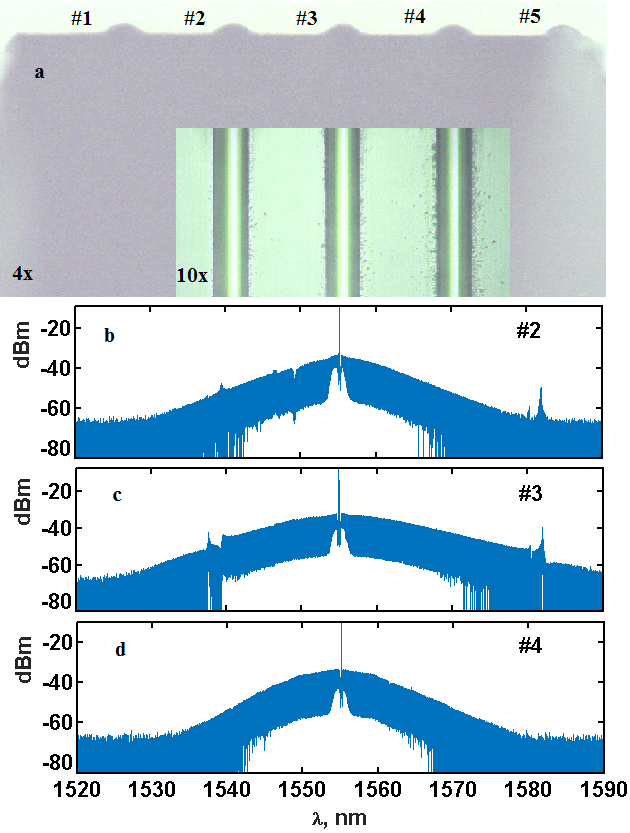
\includegraphics[width=0.75\linewidth]{dual_cavity}}
\end{minipage}
\caption{ (a): Вид резонаторов МШГ на одном кристаллическом цилиндре с диаметром 5.68 мм, радиусом кривизны 35 мкм и расстоянием между соседними выступами 140 мкм. Вставка показывает 3 неотполированные выступа (\#2 -- \#4) сразу после точения, в которых наблюдались солитоны; (b-d): оптический спектр солитонов, генерируемых в 3 различных резонаторах (\#2 -- \#4). Солитонные керровские частотные гребенки имеют ширину $30 - 65$ нм с расстоянием 12.1 ГГц.}
\label{ris:image1}
\end{figure}

Добротность после алмазного точения составила порядка 10$^6$. Сверхвысокая добротность больше $10^9$ была достигнута асимптотическим полированием алмазными суспензиями. В результате финальной полировки разница в ОСД между несколькими выступами была не более 10 МГц, что соответствует разнице в радиусе $0.5 - 1$ мкм в предположении о возбуждении одного семейства мод в обоих резонаторах.

\begin{figure}[ht]
\begin{minipage}[ht]{1\linewidth}
\center{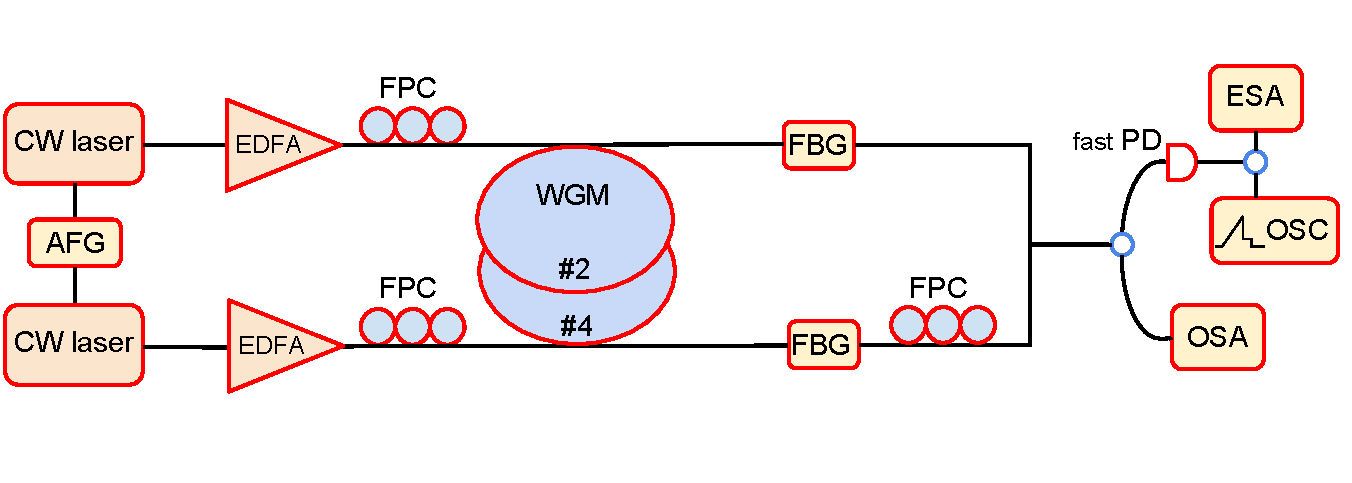
\includegraphics[width=0.75\linewidth]{dual_setup}}
\end{minipage}
\caption{Экспериментальная установка по генерации солитонных двойных гренок из выступов \#2 и \#4. CW: узкополосный перестраиваемый волоконный лазер непрерывной мощности; EDFA: эрбиевый волоконный усилитель; AFG: генератор сигналов произвольной формы; FPC:  волоконный контроллер поляризации; FBG: волоконная Брэгговская решетка; PD: фотодетектор; ESA: анализатор спектра электрических сигналов; OSA: оптический анализатор спектра; OSC: осциллограф.}
\label{ris:image2}
\end{figure}

Схема экспериментальной установке дала на Рис. \ref{ris:image2}.  Два независимых узкополосных волоконных лазера непрерывной мощности Koheras Adjustik ($\lambda \sim 1554$~нм) были усилены в эрбиевом волоконным усилителе связаны с резонаторами через 2 растянутых волокон. Каждое волокно подносится к отдельному выступу микрорезонатора (\#2 и \#4) с противоположных сторон, в которых возбуждаются солитоны с различными ОСД. Генератор сигналов произвольной формы использовался для контроля процесса возбуждения солитонов, подавая одиночный пилообразный импульс. Контроллеры поляризации использовались для оптимизации связи. Волоконная Брэгговская решетка использовались для подавления мощной накачки на выходе после микрорезонатора.

Частоты повторения солитонов наблюдались на быстром фотодетекторе (NewFocus 1014 ширина полосы 25 ГГц) и анализаторе спектра электрических сигналов (Keysight N9030). Для записи оптического спектра использовался оптический спектроанализатор (Yokogawa). На осциллографе наблюдались характерные для солитонов ступеньки в генерируемом свете.

\begin{figure}[ht]
\begin{minipage}[ht]{1\linewidth}
	\center{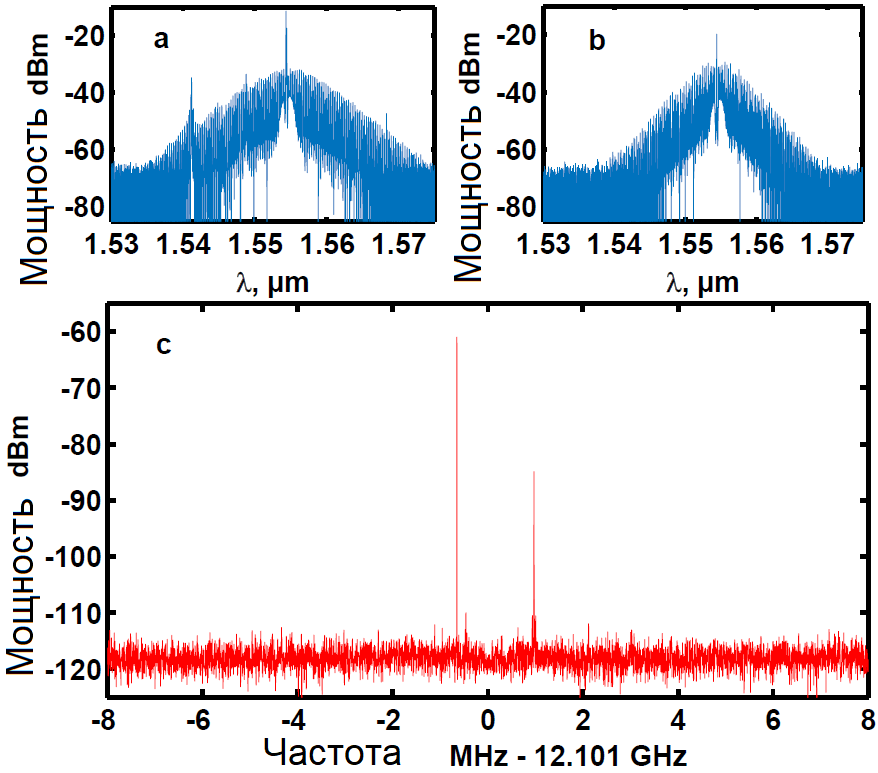
\includegraphics[width=0.5\linewidth]{dual_comb_osa}}
\end{minipage}
\caption{(a-b): Оптические мультисолитонные спектры возбужденные в двух различных резонаторах $\#2$ и $\#4$; (c): сигнал на частоте повторения от двух мультисолитоных состояний, разница в чатотах $1.62$ МГц.}
\label{ris:image3}
\end{figure}

Керровские солитонные гребенки были получены в 3 из 5 резонаторах на 1 цилиндре (Рис. \ref{ris:image1}). Ширина спектра оптических солитонов (Рис.\ref{ris:image1}(b) -- рис.\ref{ris:image1}(d)) составила 30-65 нм около 1554 нм. Разница между частотами лазеров накачки была $8.9-30$ пм. Два потока солитонов с разными частотами повторения $\Delta\mbox{FSR} = \mbox{FSR}_1 - \mbox{FSR}_2 = 1.62$~МГц были одновременно возбуждены в двух выступах на 1 кристаллическом цилиндре и далее сбиты в волоконном делители. Для настройки на солитоны использовался метод, предложенный в \cite{Herr2014}. Пилообразный однократный сигнал подавался одновременно на оба лазера, начальная точка перестройки выбиралась путем совмещения солитонных ступенек, т.ч. финальная отстройка лазеров попадала в область существования солитонов в обоих резонаторов.  

Оптические спектры мультисолитонных гребенок в обоих резонаторах даны на рис.~\ref{ris:image3}(a) -- ~\ref{ris:image3}(b), самая узкая гребенка на рис.~\ref{ris:image3}(b) содержит 350 линий, разделенных на $12.1$ ГГц и покрывает 35 нм около центральной частоты $\lambda = 1554$~нм. Разница в частотах лазеров составила $1.07$~ГГц. Результирующий сигнал биений от двух оптических гребенок переносит двойную гребенку в радиодиапазон (Рис. \ref{ris:image4}), имеет ширину 300 МГц с центром на 1.07 ГГц, содержит 160 линий, разделенных на $1.62$ МГц и имеет огибающую, совпадающую с оптическими профилями двух солитонов. Время жизни двойной гребенки была не более 30 секунд, т.к. не было стабилизации частоты лазера накачки и температуры резонатора.

\begin{figure}[ht]
\begin{minipage}[ht]{1\linewidth}
\center{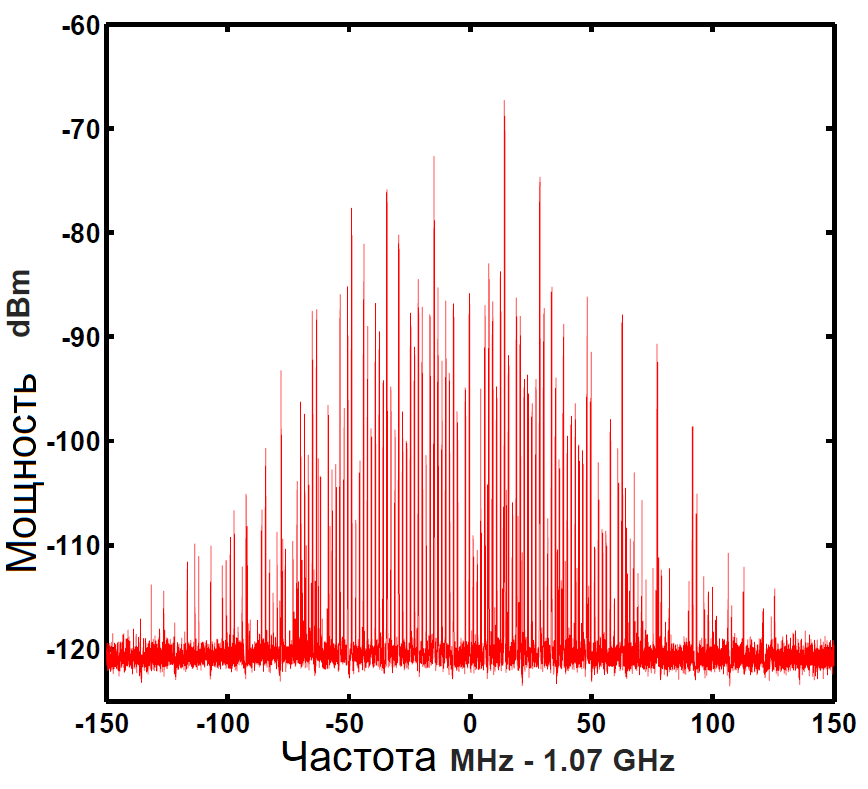
\includegraphics[width=0.5\linewidth]{dual_comb_esa}}
\end{minipage}
\caption{Радиочастотный спектр результата биений двух мультисолитонных керровских оптических гребенок. Радиочастотная двойная гребенка покрывает 300 МГц около 1.07 ГГц, содержит 160 линий, разделенных по 1.62 МГц}
\label{ris:image4}
\end{figure}

Короткое время жизни двойной гребенки обусловлено тепловым сдвигом резонансных частот. Наблюдалось, что возбуждение солитона в одном резонаторе приводило к сдвигу резонанса в другом резонаторе, т.ч. эффективная отстройка оказывалась вне области существования солитона. В результате, как правило, наблюдалось одновременное возбуждение солитона в одном резонаторе и шумной гребенки в другом резонаторе. Типичный экспериментально наблюдаемый тепловой сдвиг при возбуждении солитона в соседнем резонаторе составляет 30-50 МГц. Для уменьшения теплового влияния можно разнести резонаторы на одном цилиндре более, чем на 2 мм, использовать меньшую мощность накачки или сделать активную систему термостабилизации.

\subsection{Генерация солитонных оптических гребенок в одном резонаторе на разных семействах мод в одном направлении}

Генерация двойных оптических гребенок в отдельных резонаторах с помощью двух лазеров, не привязанных друг к другу, имеет ряд недостатков: необходимость изготавливать два одинаковых резонатора с высокой добротностью и разницей в диаметрах на уровне единиц микрон, удваивается количество оптических элементов в экспериментальной установке - требуются дополнительные изоляторы, контроллеры поляризации и оптические делители. Необходимо стабилизировать температуру обоих резонаторов. Даже при реализации всего вышеперечисленного результирующий сигнал двойной гребенки в радиодиапазоне имеет мгновенную ширину индивидуальной линии порядка 500 кГц и нестабильность частоты порядка 50 МГц на временах 10 с, обусловленного в основном нестабильностью частот лазеров накачки и различными тепловыми флуктуациями двух независимых резонаторов.

Все изготовленные в ходе работы резонаторы из $MgF_2$ были многомодовыми. Общее количество мод можно уменьшать, увеличивая соотношения радиуса цилиндра к радиусу кривизны боковой грани. Наименьшее количество мод на одну ОСД было в резонаторах диаметром 5.6 мм и радиусом кривизны 35 мкм и в резонаторе 7.5 мм диаметром и 80 мкм радиусом кривизны. При этом при хорошей полировке наблюдалось несколько семейств мод с добротностью порядка $10^9$. 

Пример сканирования широкоперестраиваемым лазером большой мощности ОСД резонатора из $MgF_2$ дан на рис. \ref{Scan_SolitonSpot}, видно возбуждение гребенок на значительном количестве семейств мод, при этом характерные солитонный ступеньки в генерируемом свете видны на меньшем числе мод, они помечены черным и даны в увеличенном масштабе. Резонатор имел диаметр около 5.5 мм и радиус кривизны боковой поверхности 80 мкм (Рис. \ref{Figure1_V1_c} (a)).

\begin{figure}[ht]
\begin{minipage}[ht]{1\linewidth}
\center{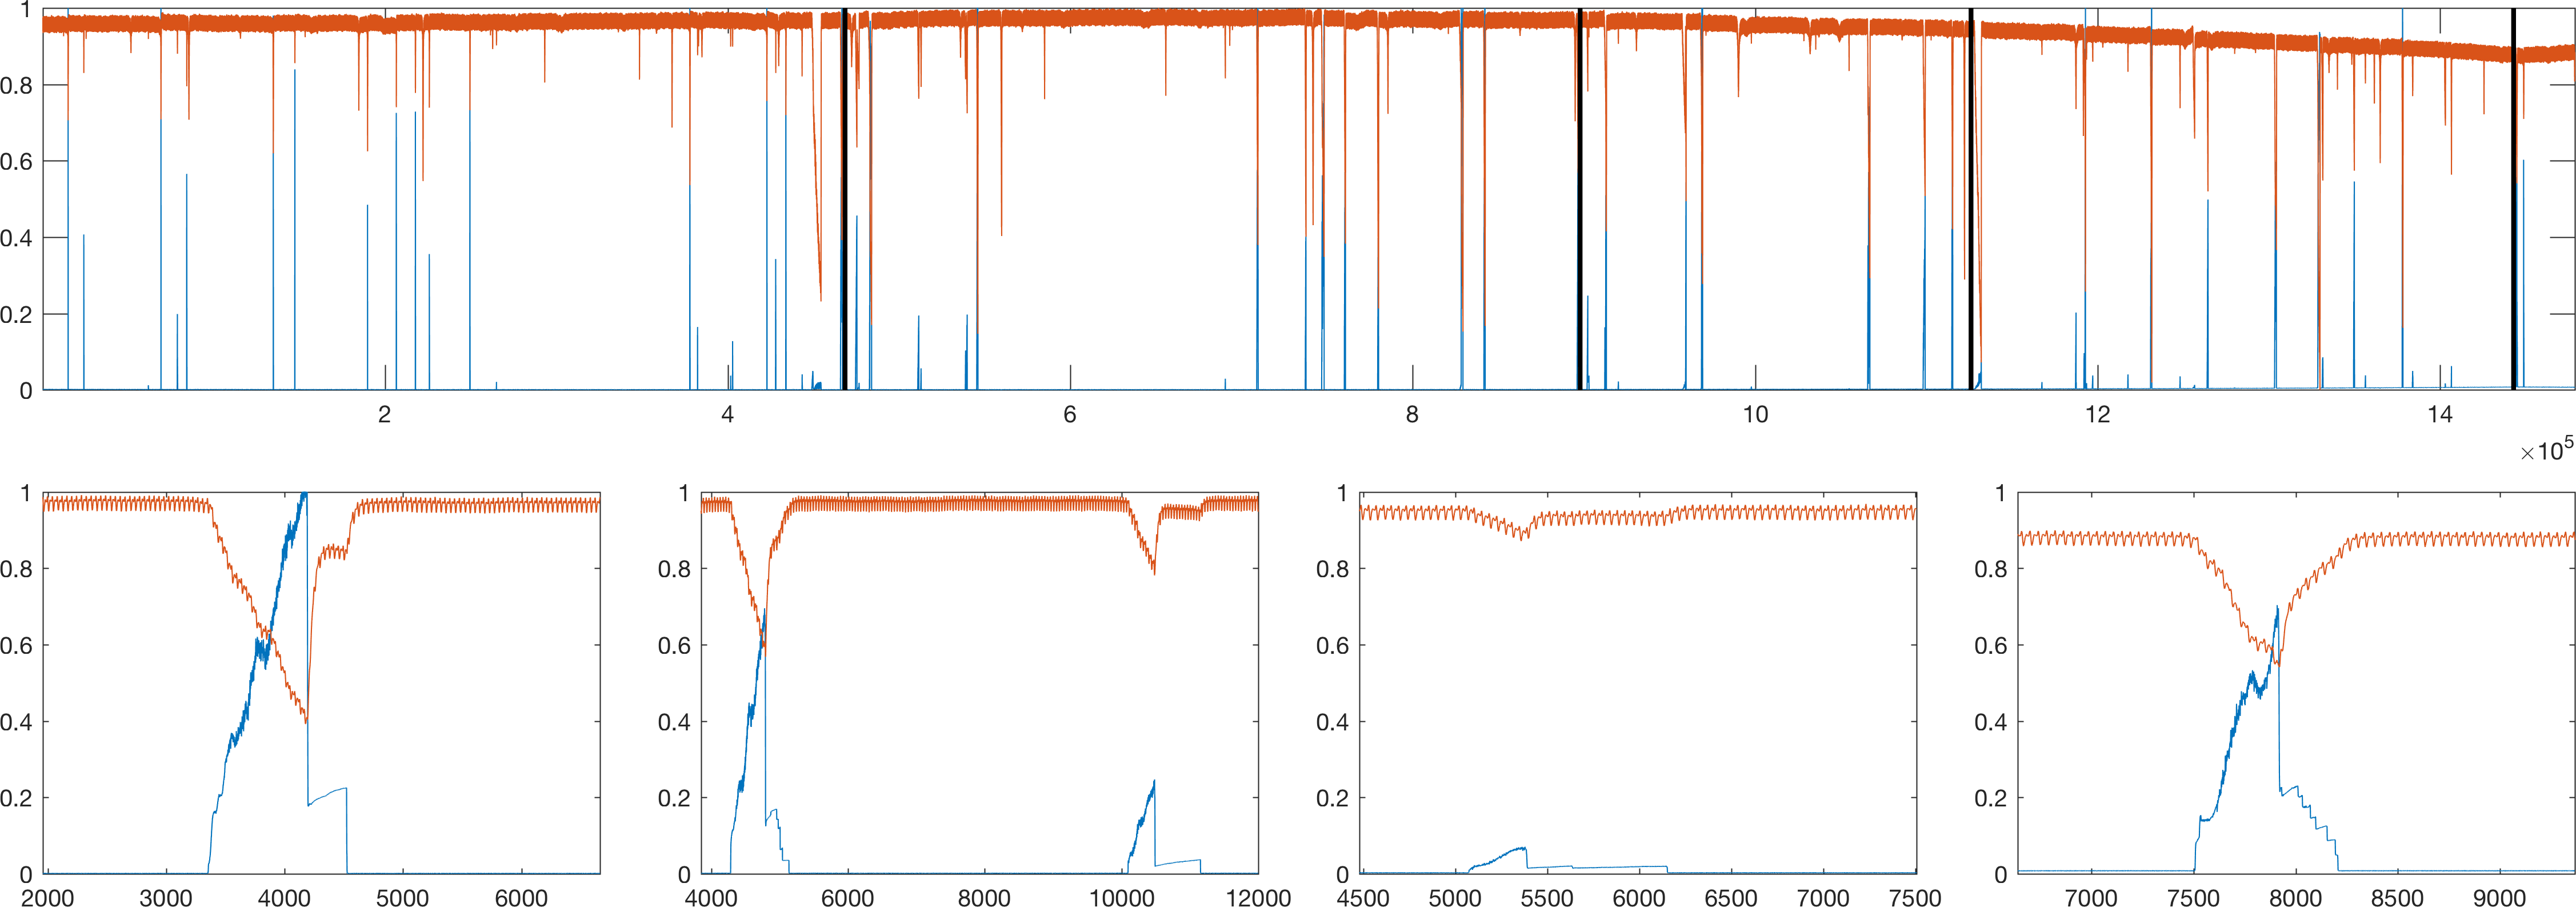
\includegraphics[width=1\linewidth]{Scan_SolitonSpot}}
\end{minipage}
\caption{Сканирование лазером большой мощности 1 ОСД резонатора из $MgF_2$. Сверху красным даны сигналы пропускания системы, синим - генерируемый свет (сигнал пропускания за вычетом отфильтрованного мощного сигнала накачки). Наблюдается большое количество оптических гребенок, генерируемых на разных семействах мод. Черным выделены несколько примеров мод с характерным для генерации солитонов ступеньками в сигнале генерируемого света (даны в увеличенном масштабе в нижнем ряду)}
\label{Scan_SolitonSpot}
\end{figure}

Был проведен эксперимент по одновременной генерации солитонов на разных семействах мод (Рис. \ref{Figure1_V1_c}), т.ч. одно семейство мод накачивалось лазером, а другое семейство боковой линией амплитудной модуляции этого лазера. Использовался амплитудный модулятор с 1 боковой линией, сигналы от которых усиливались в эрбиевом волоконном усилителе. Связь с резонатором осуществлялась через одно растянутое волокно. Сигнал на выходе системы проходил через волоконный Брэгговский фильтр для подавления мощного сигнала накачки и анализировался на оптическом спектроанализаторе и быстром фотодиоде с помощью анализатора сигналов. Частота сигнала, подаваемого на модулятор выбиралась так, чтобы на картине сигнала генерируемого света, ступеньки от двух нелинейных резонансов совпадали, их пересечение является областью одновременного существования солитонов (Рис. \ref{Figure2}). Далее использовалась стандартная техника настройки на солитонный режим, когда подается однократный пилообразный сигнал, который быстро перестраивает лазер в область существования солитонов. Использовалась активная температурная стабилизация резонатора с помощью элемента Пельтье, установленного под подставку под резонатора, диодный датчик температуры, который был закреплен на подставке (не на резонаторе, что вносило дополнительную задержку при стабилизации) и PID регулятор. Температура резонатора стабилизировалось с точностью до 10 мК. Стабилизация отстройки частоты лазера проводилась методом PDH.

\begin{figure}[ht]
\begin{minipage}[ht]{1\linewidth}
\center{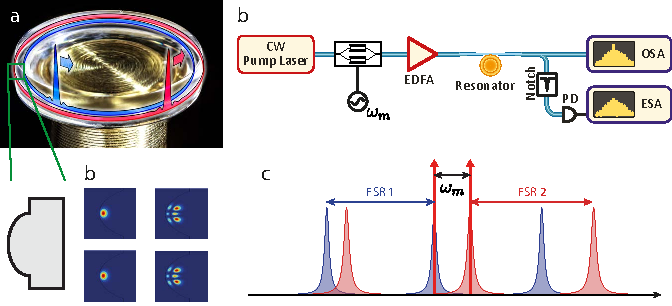
\includegraphics[width=0.75\linewidth]{Figure1_V1_c}}
\end{minipage}
\caption{(а) Фотография резонатора $MgF_2$ диаметр 5.5 мм, радиус кривизны боковой поверхности 80 мкм, схематично изображены 2 солитона на различных семействах мод, распространяющихся в одном направлении, ниже даны примеры распределения поля внутри МШГ для 2х разных семейств мод, (b) Схема экспериментальной установки: CW pump laser - волоконный перестраиваемый лазер непрерывной мощности, волоконный амплитудный модулятор с 1 боковой линией, EDFA - эрбиевый волоконный усилитель, резонатор из (а), Notch - волоконный Брэгговский фильтр, PD - быстрый фотодиод, OSA - оптический спектроанализатор, ESA - анализатор спектра электрических сигналов. (с) концептуальная схема эксперимента, красным и синим изображены разные пространственные семейства мод в одном резонаторе, имеющие разные ОСД FSR1 и FSR2, расстояние между накачиваемыми двумя модами $\omega_m$ выбирается как частота модуляции.}
\label{Figure1_V1_c}
\end{figure}

\begin{figure}[ht]
\begin{minipage}[ht]{1\linewidth}
\center{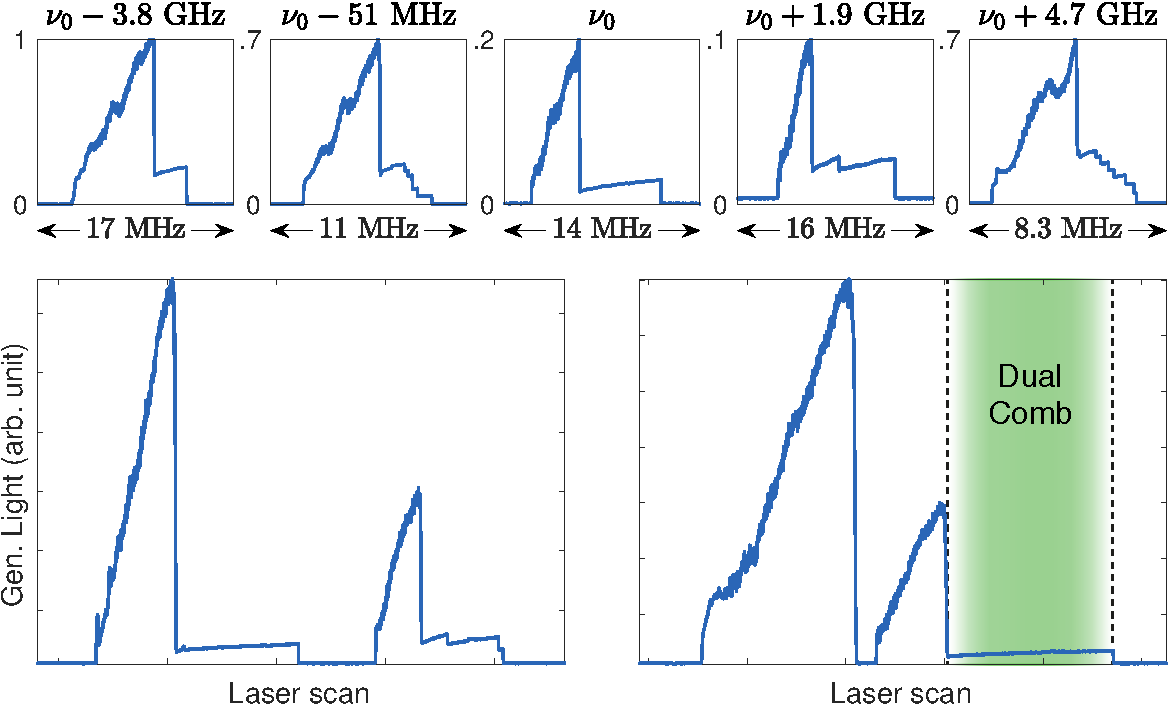
\includegraphics[width=0.5\linewidth]{Figure2}}
\end{minipage}
\caption{Сверху показаны сигналы генерируемого света для разных семейств мод, содержащие характерные солитонные ступеньки, даны отличия собственных частот для этих мод от выбранной центральной. Масштаб по вертикальной оси разный. Внизу показан метод совмещения солитонных ступенек при изменении частоты модуляции. Зеленой областью показан диапазон отстройки, при котором одновременно могут существовать солитоны на обоих семействах мод.}
\label{Figure2}
\end{figure}

В ходе эксперимента удалось одновременно настроиться на оба солитона на разных семействах мод и стабилизировать отстройку частоты лазера, т.ч. солитоны существовали несколько часов. На рис. \ref{Co_Scheme_results} приведены экспериментальные результаты по одновременной генерации односолитонных режимов на двух разных семействах мод в одном резонаторе. Амплитуда лазера и 1 линии боковой модуляции были сделаны одинаковыми, частота модуляции составила 4.2817 ГГц, на этой же частоте наблюдалась результирующая гребенка в СВЧ диапазоне. Расстояние между линиями СВЧ гребенки составила 655 кГц, что равно разнице между частотами повторения солитонов на двух семействах мод. С помощью быстрого фотодетектора и осциллографа был измерена интерферограмма, которая подтвердила, что в результате мультигетеродинирования двух оптических солитонов образовался импульс в СВЧ диапазоне, огибающая которого соответствует огибающим в оптическом диапазоне. Также была измерена ширина одной нецентральной линии СВЧ гребенки, она составила 100 Гц, что говорит об очень высокой взаимной когерентности оптических солитонов, которая в данном случае определяется стабильностью подаваемого СВЧ сигнала на модулятор и качеством стабилизации частоты отстройки лазера. 

Таким образом был продемонстрирован перенос 35 нм оптической гребенки с центром на 1554 нм в СВЧ область с центром на 4.28 ГГц и шириной около 200 МГц. Такой источник двойной гребенки может использоваться для спектроскопии и быстрого измерения расстояний.

\begin{figure}[ht]
\begin{minipage}[ht]{1\linewidth}
\center{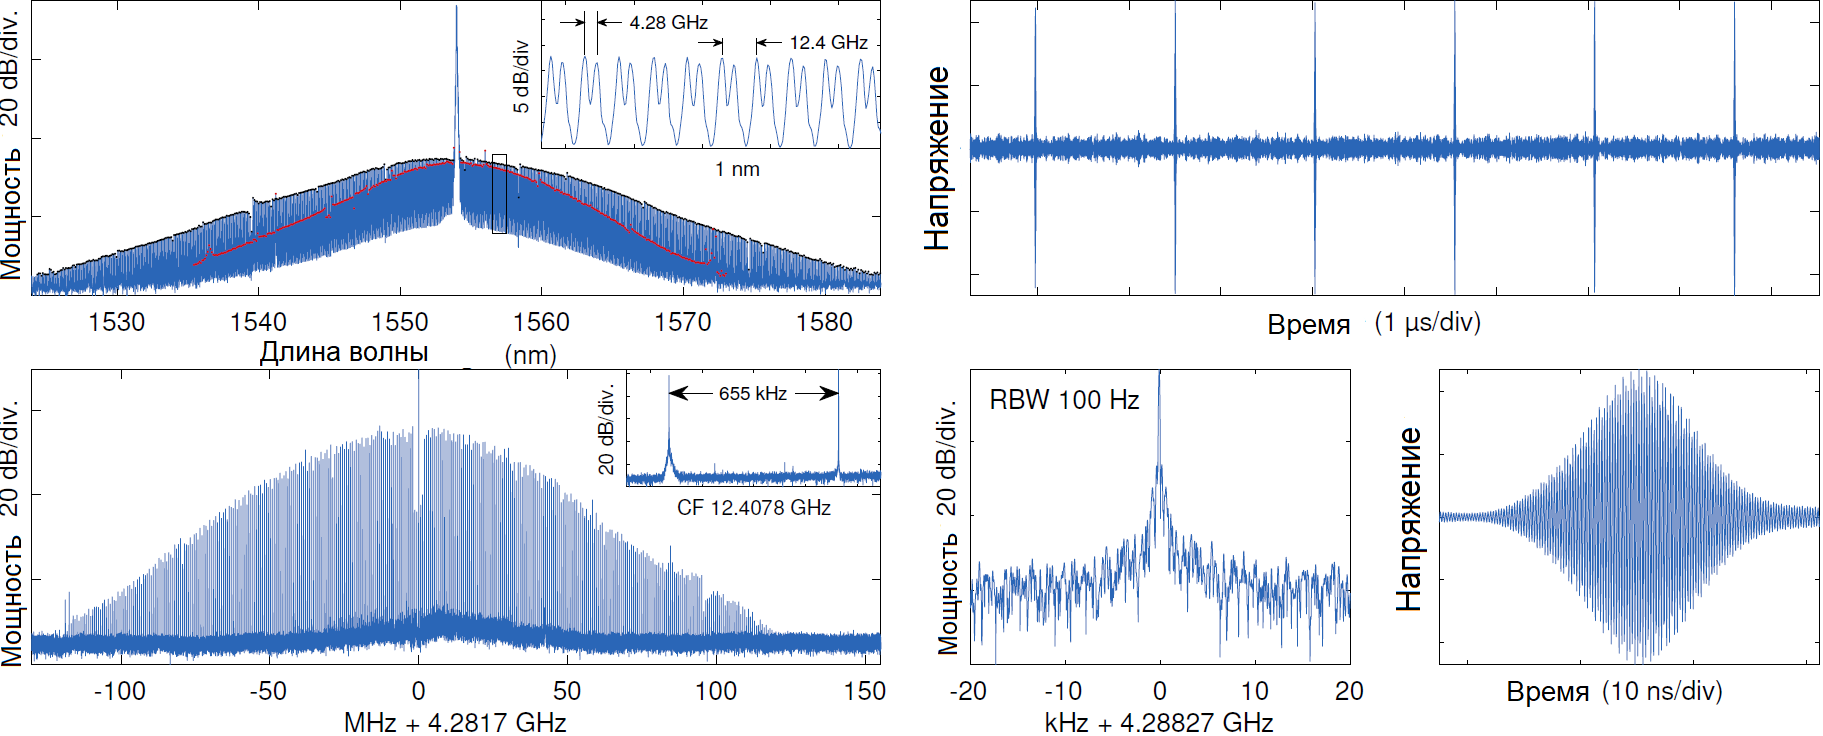
\includegraphics[width=1\linewidth]{Co_Scheme_results}}
\end{minipage}
\caption{Экспериментальные результаты одновременного возбуждения односолитонных режимов на двух разных семействах мод в 1 микрорезонаторе. (а) суммарный оптический спектр односолитонных режимов, красной линией помечена огибающая второго солитона, на вставке представлены отдельные линии двух солитонов. ОСД резонатора 12.4 ГГц, расстояние между несущими 4.28 ГГц. (b) результирующий сигнал биений двух солитонов - СВЧ гребенка с расстоянием между линиями 655 кГц, которое соответсвует разнице между ОСД семейств мод, на вставке изображены сигналы частот повторения двух солитонов, (с) сигнал последовательности результирующих СВЧ импульсов, снятый быстрым осциллографом ,(d) одиночная нецентральная линия СВЧ гребенки шириной около 100 Гц, (е) сигнал одиночного СВЧ импульса, соответствующий СВЧ гребенки}
\label{Co_Scheme_results}
\end{figure}

На рис. \ref{coscheme_different_types} приведены результаты генерации солитонов на другой паре семейств мод. Частота модуляции, равная разнице собственных частот мод из двух семейств, составила $4.9119$~ГГц, расстояние между ОСД семейств мод 9.2633~МГц, оно же являлось расстоянием между линиями СВЧ гребенки. В данном случае на одном семействе мод был достигнут односолитонный режим, а на другом многосолитонный. Хорошо видно совпадение огибающих оптического спектра солитонов и результирующего спектра СВЧ сигнала. Отметим видимый в этом эксперименте недостаток, при большом отличие ОСД между семействами мод, результирующая СВЧ гребенка перекрывается с собой, т.к. линии от мультигетеродинирования расположены вокруг центральных частот $\omega_m$ и $FSR-\omega_m$. Этот же недостаток может проявляться и при достаточно малых $\omega_m$.

Измерение стабильности индивидуальной линии \ref{single_line_stability_cp} говорит о хорошей стабилизации частоты лазера накачки и температуры резонатора.

\begin{figure}[ht]
\begin{minipage}[ht]{1\linewidth}
\center{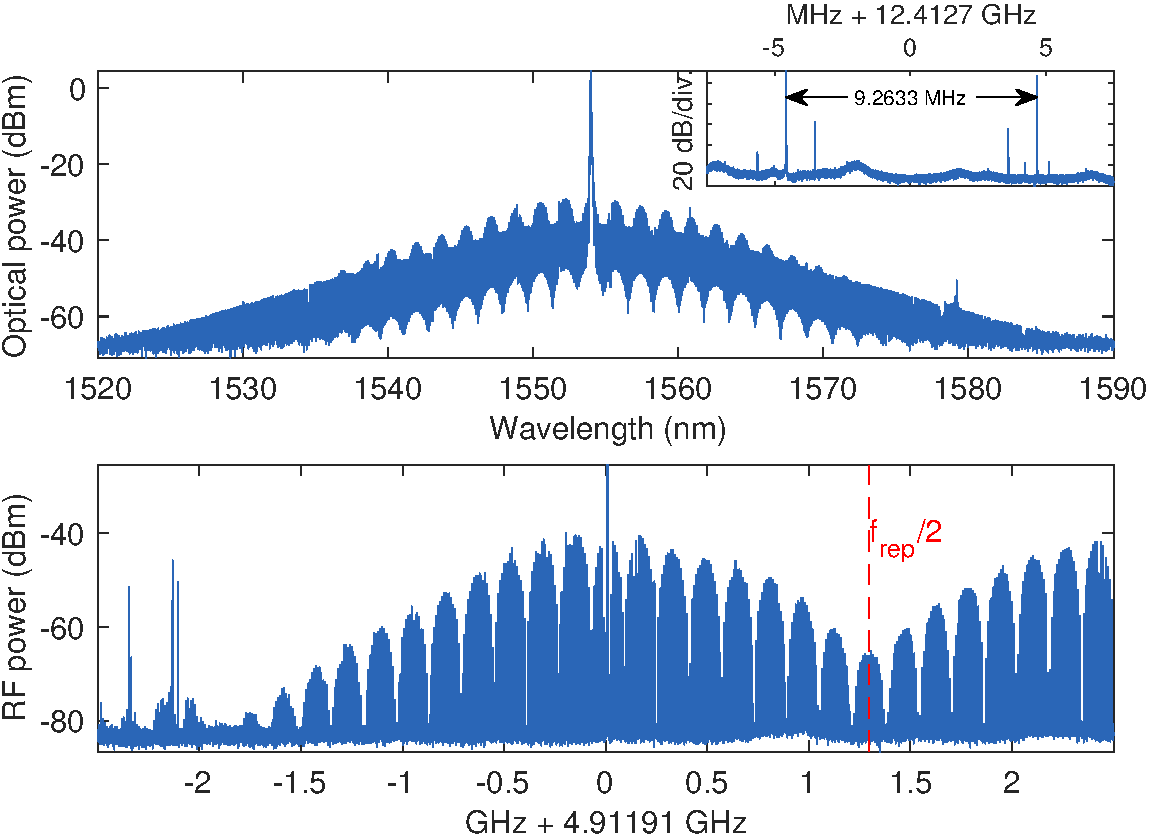
\includegraphics[width=0.75\linewidth]{coscheme_different_types}}
\end{minipage}
\caption{Результаты генерации солитонов в одном направлении на другой паре семейств мод. (а) суммарный оптический спектр односолитонного режима на одном семействе мод и многосолитонного режима на другом семействе мод, на вставке показана разница между частотами повторений 9.2633~МГц, (b) результирующая CВЧ гребенка с центральной частотой 4.9119 ГГц, видно что гребенка перекрывается с собой на половине частоты повторонения солитонов, отмечено красной линией.}
\label{coscheme_different_types}
\end{figure}

\begin{figure}[ht]
\begin{minipage}[ht]{1\linewidth}
\center{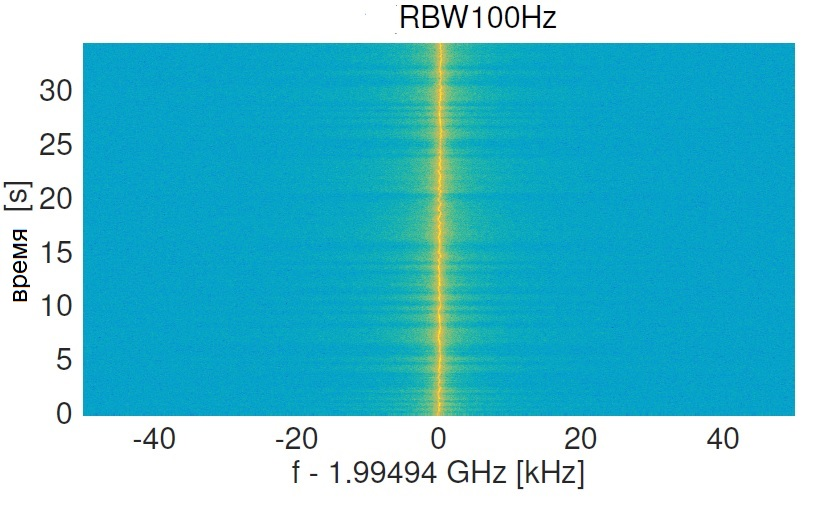
\includegraphics[width=0.5\linewidth]{single_line_stability_cp}}
\end{minipage}
\caption{Измерение стабильности индивидуальной линии СВЧ гребенки.}
\label{single_line_stability_cp}
\end{figure}

Отметим также технический недостаток схемы с двумя солитонами в одном направлении - сигнал ошибки схемы PDH несет информацию одновременно от обоих резонансов, что может мешать стабилизации, особенно при наличии эффекта пересечения мод хотя бы на одном солитонном резонансе.

Практическим для некоторых приложений недостатком схемы с двумя солитонами в 1 направлении является невозможность разделить эти солитоны (у них одна поляризация и близкие частоты линий), поэтому такая схема может не подойти, например, для фазово-чувствительной спектроскопии поглощения веществ. Отметим, что признаков взаимодействия солитонов в данном эксперименте не было обнаружено.

\subsection{Генерация солитонных оптических гребенок в одном резонаторе на разных семействах мод в противоположных напрвлениях}

Чтобы разделить солитоны из одного резонатора был проведен следующий эксперимент, в котором солитоны на разных семействах мод возбуждались в противоположных направлениях. Схема экспериментальной установки приведена на рис. \ref{Setup_CounterProp}. Волоконный перестраиваемый лазер непрерывной мощности усиливается эрбиевым усилителем, 0.1 мощности в одном плече после делителя модулируется амплитудным модулятором с одной боковой линией в таком режиме, что вся мощность перекачивается в эту боковую линию, далее сдвинуты по частоте лазерный сигнал усиливается и подается через циркулятор в резонатор из $MgF_2$, другое плечо содержит 0.9 мощности исходного лазера и подается через другой циркулятор на тот же элемент связи - растянутое волокно. Третьи выходы двух оптических циркуляторов в такой конфигурации содержат свет, прошедший через резонатор в противоположных направлениях. Брэгговские волоконные фильтры используются для подавления мощных несущих. Далее полученные сигналы независимо подаются на оптические спектроанализаторы и могут быть сбиты на волоконном делителе и отправлены на быстрый фотодетектор для генерации СВЧ гребенки.

\begin{figure}[ht]
\begin{minipage}[ht]{1\linewidth}
\center{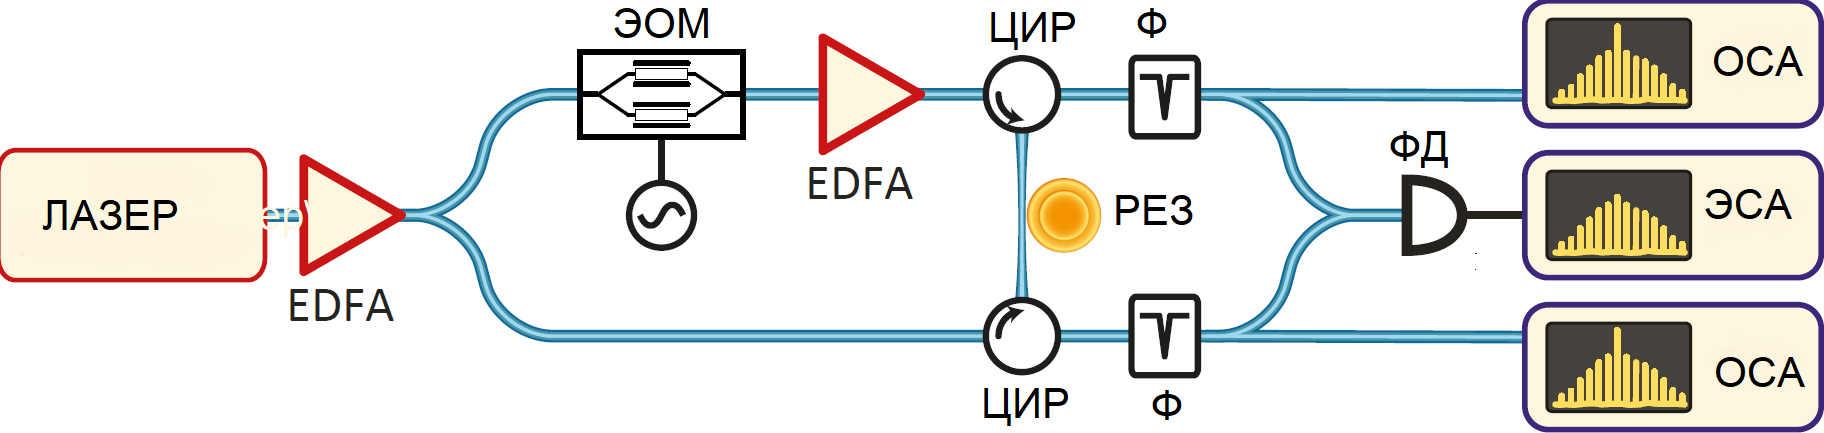
\includegraphics[width=0.75\linewidth]{Setup_CounterProp}}
\end{minipage}
\caption{Схема экспериментальной установки: CW pump laser - волоконный перестраиваемый лазер непрерывной мощности, волоконный амплитудный модулятор с 1 боковой линией, EDFA - эрбиевый волоконный усилитель, резонатор из (а), Notch - волоконный Брэгговский фильтр, PD - быстрый фотодиод, OSA - оптический спектроанализатор, ESA - анализатор спектра электрических сигналов, CIR - оптический циркулятор}
\label{Setup_CounterProp}
\end{figure}

В эксперименте мощность накачек в обоих плечах выравнивалась, а частота модуляции подбиралась так, чтобы совпадали солитонные ступеньки в сигнале генерируемого света, также как и в случае солитонов в 1 направлении на разных семействах мод. Использовался метод PDH стабилизации частоты лазера к моде резонатора. Также была задействована схема активной стабилизации температуры резонатора. Экспериментальные результаты приведены на \ref{counter_prop_results}. Красный оптический спектр имеет сильно выраженный пик на 1530 нм, вероятно, связанный с сильным эффектом пересечения мод. Результирующая картина СВЧ гребенки хорошо воспроизводит огибающие оптических спектров солитонов (однако присутствуют дополнительные компоненты на +70 МГц и -70 МГц вероятно связанные с техническими шумами). Результаты измерения девиации Аллана показывают, что разница частот повторений солитонов стабильнее, чем индивидульная частота биений для 1 солитона, что говорит о хорошей работе системы привязки PDH. Для того чтобы минимизировать флуктуации амплитуд индивидуальных линий СВЧ гребенки необходимо бороться с паразитными переотражениями в схеме после резонатора, иначе образуются дополнительные резонаторы типа Фабри-Перо, и избегать флуктуаций фазы света в плечах, уменьшая длину волокон и контролируя их температуру и механические вибрации. 

Продемонстрированный метод генерации двойной гребенки в противоположных направлениях на разных семействах мод подходит для проведения фазочувствительной спектроскопии. Отметим, что признаков взаимодействия солитонов в данном эксперименте не было обнаружено. 

\begin{figure}[ht]
\begin{minipage}[ht]{1\linewidth}
\center{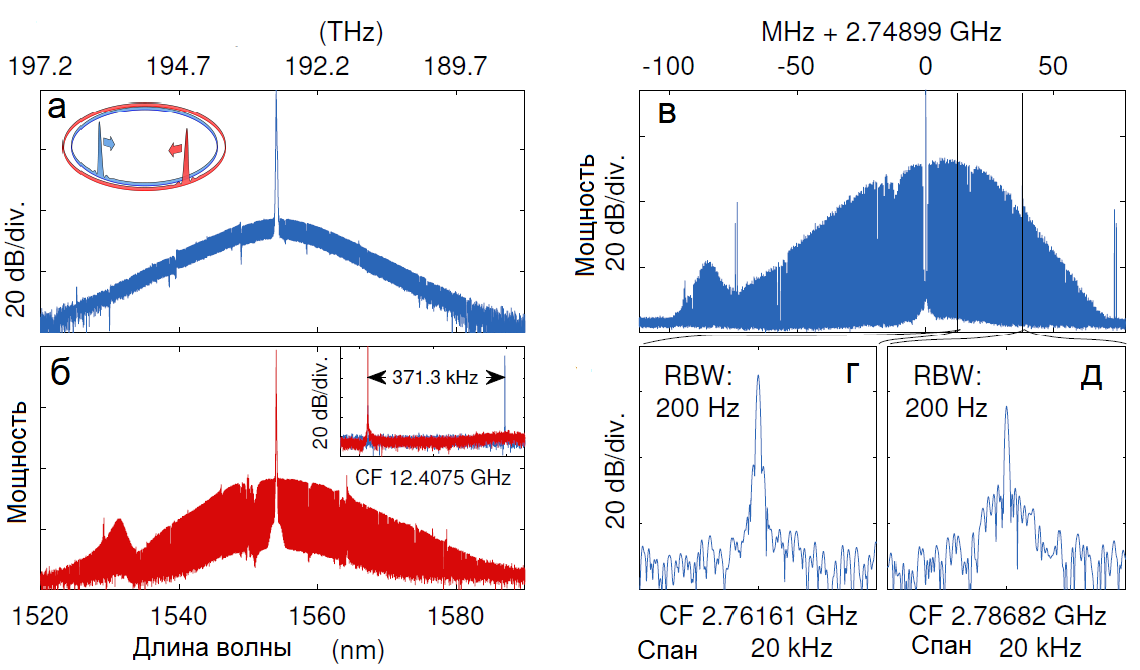
\includegraphics[width=1\linewidth]{counter_prop_results}}
\end{minipage}
\caption{Экспериментальные результаты возбуждения солитонов в противоположных направлениях в 1 резонаторе на разных семействах мод. (а,с) Оптические спектры односолитонных режимов, полученных на разных семействах. На вставке показаны наложенные друг на друга сигналы биений на частоте повторения солитонов. Разница в частотах повторений составила 371 кГц. (b) Результирующая СВЧ гребенка при совмещении потоков солитонов, распространяющихся в противоположном направлении, центральная частота совпадает с частотой модуляции 2.748 ГГц, расстояние между линиями 371 кГц, (d) измерение девиации Аллана частоты повторения для одного потока солитонов на 12.407 ГГц (красные точки) и для их разности (черные точки)}
\label{counter_prop_results}
\end{figure}

\subsection{Генерация солитонных оптических гребенок в одном резонаторе на одном семействе мод в противоположных напрвлениях}

Предложенный метод генерации солитонов в 1 резонаторе в противоположных направлениях применим не только при накачке разных семейств мод, но возможен и на одном семействе мод. Используя схему \ref{Setup_CounterProp} и экспериментальный метод из предыдущего раздела, возможно возбудить два солитона на 1 моде в противоположных направлениях \ref{cp_one_family}, для этого на амплитудный модулятор подается частота не выше максимальной отстройки, при которой существует солитон (типичные значения 5-20 МГц). Т.к. частота повторения солитонов зависит от отстройки частоты накачки от холодного резонанса, то при небольшом сдвиге накачки в прямом и обратном направлениях возможно образование результирующей СВЧ гребенки \ref{cp_one_family_dual_comb}. Важно отметить, что существует пороговое значение этой отстройки (частота на модуляторе менее 2 МГц), при которой частоты повторения солитонов строго совпадают и двойная гребенка не наблюдается. Также экспериментально обнаружено, что частоты повторений могут совпасть и при таком значении отстройки, когда возбуждаются сильные пересечения мод. Важно отметить, что использования одного лазера недостаточно, т.к. при 0 отстройке накачек друг относительно друга, частоты повторений совпадают.

Измеренная стабильность индивидуальных линий \ref{cp_one_family_stability} показывает дрифт на 100 Гц за 60 сек, однако флуктуации амплитуды индивидуальных линий были высокими (Рис. \ref{cp_one_family_dual_comb} (b)), вероятной технически устранимой причиной являются сильные паразитные переотражения на коннекторах волокон волоконного делителя.

\begin{figure}[ht]
\begin{minipage}[ht]{1\linewidth}
\center{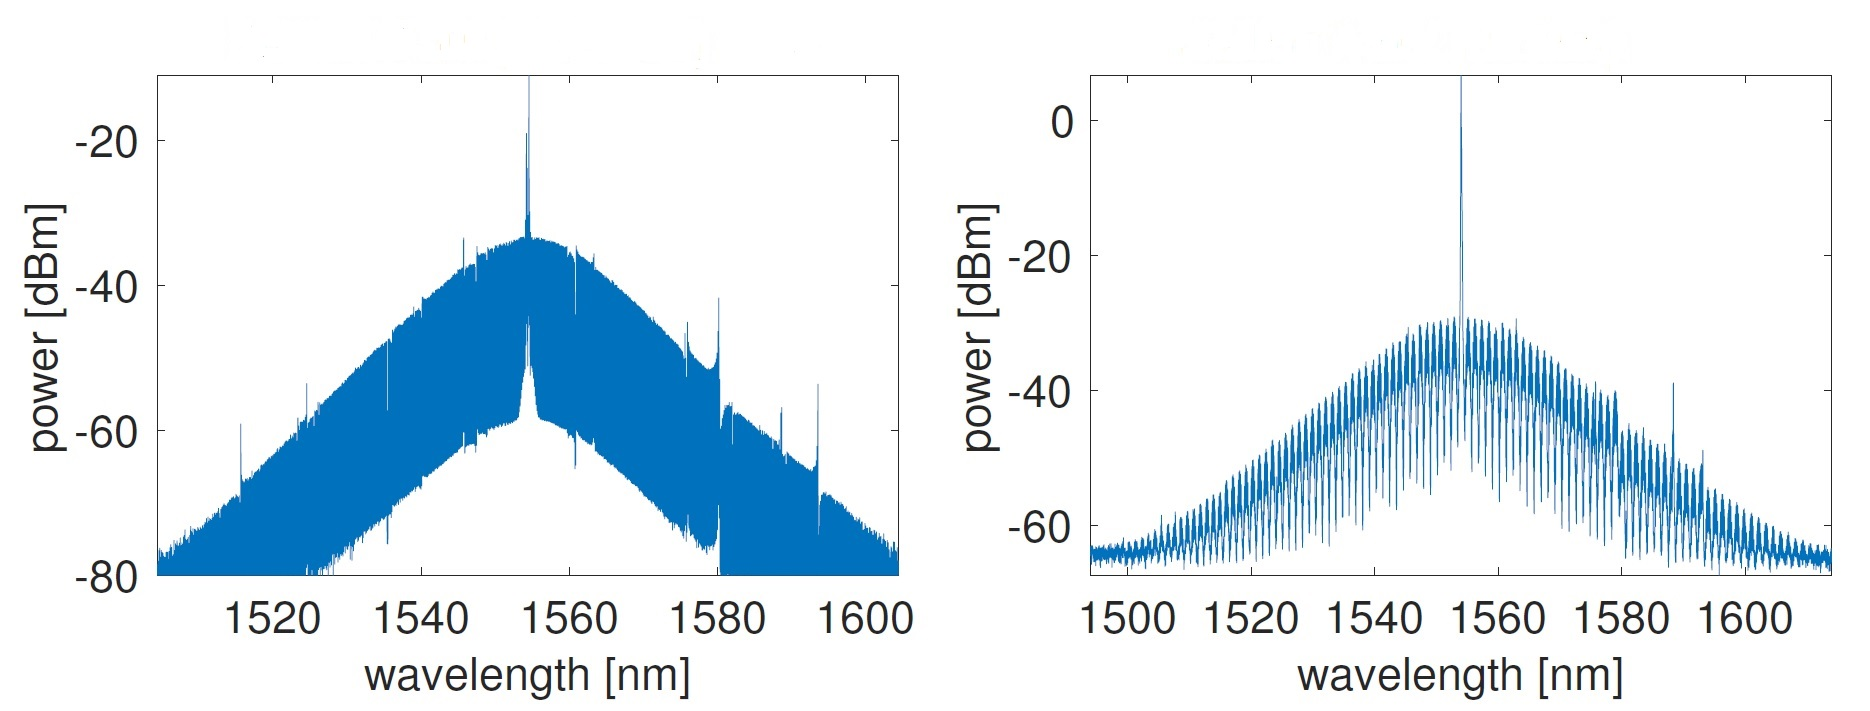
\includegraphics[width=0.7\linewidth]{cp_one_family}}
\end{minipage}
\caption{Экспериментальные результаты возбуждения солитонов в противоположных направлениях в 1 резонаторе на одном семействе мод. (а,b) Оптические спектры: односолитонный режим в одном направлении, многосолитонный режим в противоположном направлении на том же семействе мод.}
\label{cp_one_family}
\end{figure}

\begin{figure}[ht]
\begin{minipage}[ht]{1\linewidth}
\center{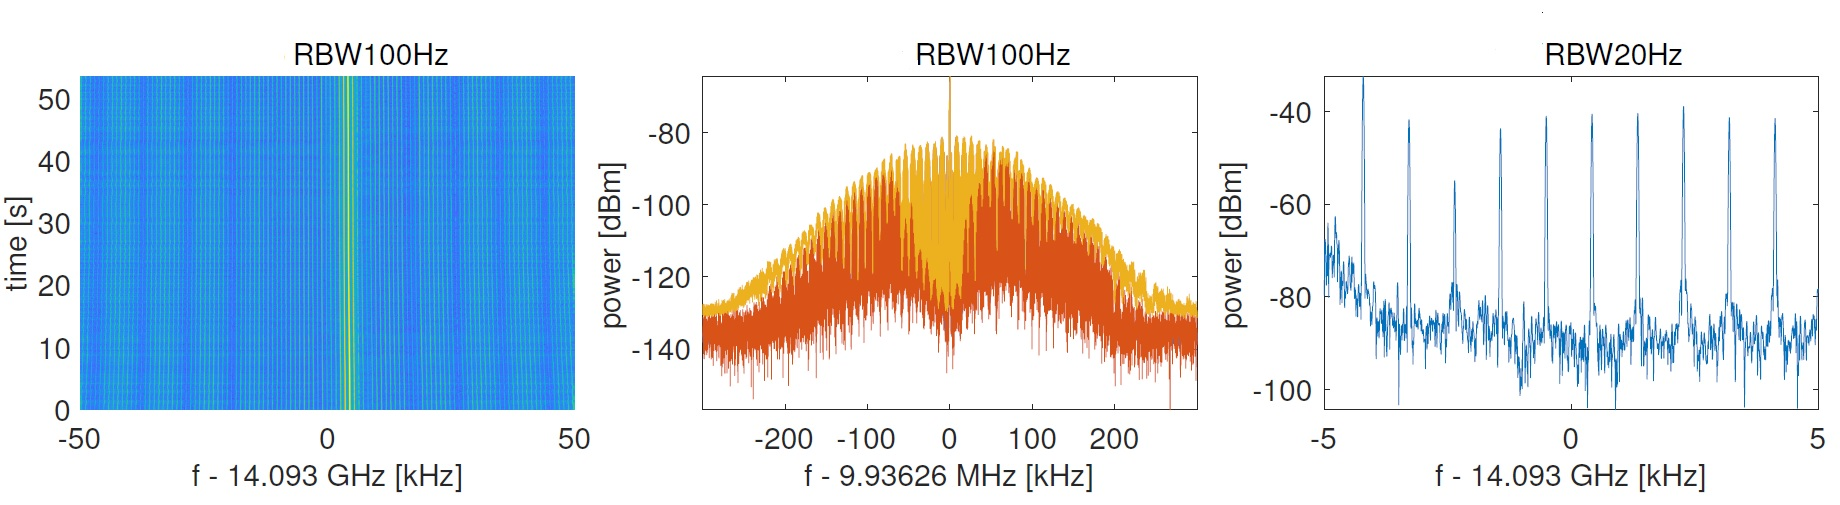
\includegraphics[width=1\linewidth]{cp_one_family_dual_comb}}
\end{minipage}
\caption{Результирующая СВЧ гребенка при совмещении потоков солитонов, распространяющихся в противоположном направлении, центральная частота совпадает с частотой модуляции 9.93 МГц, расстояние между линиями СВЧ гребенки порядка 1 кГц и растет с увеличением разности частот накачек. (а) стабильность результирующей гребенки, (b) спектр гребенки, желтым максимальное значение, красным - усредненное за 10 сек, (c) спектр индивидуальных линий результирующей гребенки}
\label{cp_one_family_dual_comb}
\end{figure}

\begin{figure}[ht]
\begin{minipage}[ht]{1\linewidth}
\center{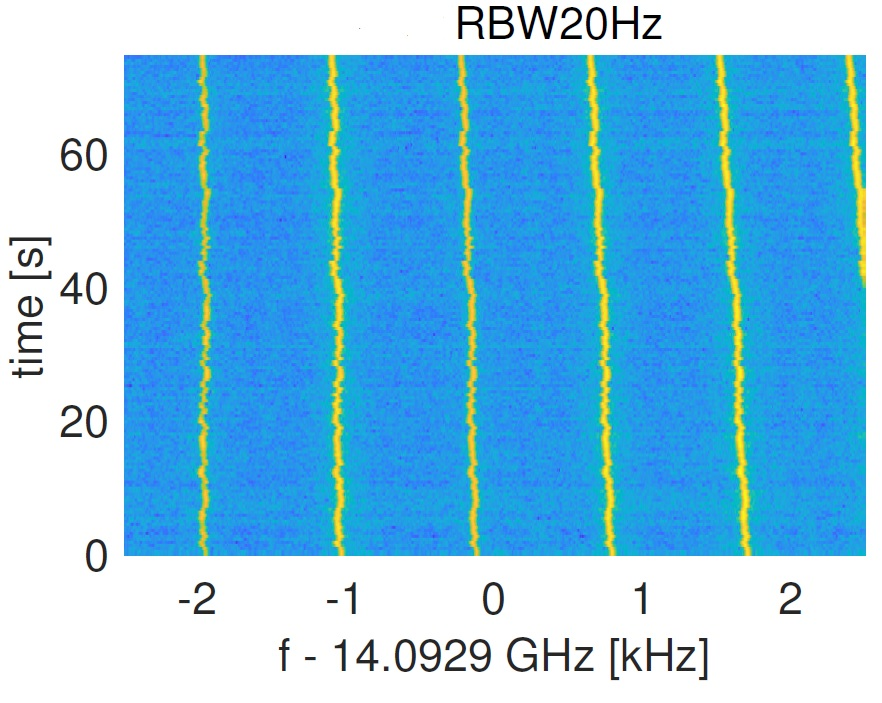
\includegraphics[width=0.5\linewidth]{cp_one_family_stability}}
\end{minipage}
\caption{Стабильность индивидуальных линий гребенки, полученной как биение двух солитонов, возбужденных на одном семействе мод в противоположных направлениях}
\label{cp_one_family_stability}
\end{figure}

Предложенный метод может быть удобен тем, что подходит для одномодовых резонаторов или резонаторов, не поддерживающих солитоны на разных семействах мод, а также тем, что не требует высоких частот, подаваемых на модулятор и быстрых фотодетекторов для регистрации двойных гребенок в СВЧ области.

Сошлемся на все конференции \cite{confbib1,confbib2,confbib3,confbib4,confbib5,confbib6,confbib7,confbib8,confbib9,confbib10,confbib11,confbib12,confbib13,confbib14} 
%\section{Экспериментальное наблюдение вынужденного рассеяния Рамана и Бриллюэна в кристаллических микрорезонаторах}